\chapter{Information Gathering}\label{InformationGathering}
This section collects information about meal planning and food waste. Food waste will be examined by, first using general statistics and then, by using different reports to understand peoples perception of food waste. Meal planning is also examined, by using different reports to get an understanding of how people plan meals, and what difficulties that are associated with this task. 
 
\section{Food waste}
Every year danish households throws away nearly 237.000 tons of food, that could have been eaten by people. This is estimated to be nearly 16 mio DKK. About 20 \% of a danish households foodbudget is wasted by throwing away food that could have been eaten, this means that if there was no food waste at all, 1 million people could be fed, this is nearly 1/5 of the danish people.

The people who throws away most food, are the people living alone. The average person living alone throws away 98.8 kg of food per year, where as a household with 5 people throws away 46.8 kg of food per person per year. It is mostly dairy products, vegetables and bread that gets thrown away, though in december a lot of meat is also thrown away, due to the fact that it is Christmas, where people eat more food.

Since 2007 the danish people have been purchasing 10 \% less food, a lot of this food used to end up in the trashcan as food waste. 54 \% of the danish people rarely or never uses the food from the night before for later eating, and 69 \% does not use leftovers for lunch the day after. Elderly people are better at using leftovers than younger people. \fxnote{references to bibliography, and/or maybe some graphs to show the numbers?}

20 \% of danish people does not make a grocery shopping list before going grocery shopping. 52 \% of people does not make a meal plan, 31 \% does sometimes and 17 \% does it often.

81 \% of danish people would use leftovers to avoid food waste, 50 percent would make a mealplan and make a grocery shopping list. 59 \% of the consumers believe that the danish food waste is their own fault.

\section{FDB Report}
The following section examines a report published in 2011 by FDB called "Forbrugerne: Vi smider ikke mad ud"\cite{madSpild_FDB}.
\subsection{Method used in the report}
The report is an anthropological study of how food waste occurs and how it is experienced by the consumers. The study is based on qualitative data collected from six different households. These households are all different from one another e.g. they live in different geographical locations. Data is gathered from the participants by using observations e.g. watching participants shop or prepare food, semi-structured interviews and probing kits. The data is then used to examine the activity patterns and motivation of the participants.

\subsection{FDB report: What is food waste and how does it occur.}
The report discusses why food waste occurs and how the participants perceive it. There are some subjects that are interesting when learning about food waste. 

\subsubsection{What is food waste}
When the participants was asked how much food they threw out, they typically answered that they threw out as little as possible. There is a clear distinction between waste and non-waste being thrown out. It is acceptable to throw waste out, but not to do the same with non-waste. The waste and non-waste categories varies depending on cooked food products and uncooked food products. Cooked food is considered waste when larger parts, or leftovers of a meal that has not been served on a plate is thrown out. So when the food has been served on a plate it is acceptable to throw it out. Uncooked food is considered waste when the packaging is unopened. It is not considered waste when the uncooked fat or other food parts that are considered non-edible is thrown out.

\subsubsection{Cause of food waste} 
The reasons as to why food is thrown out varies depending on cooked and uncooked products. Uncooked products is thrown out because they are bought in so large quantities that the consumers were not able to eat it prior to expiry. Products that are considered non-edible such as cartilage or bad vegetables are also thrown out. Cooked food products are also likely to be thrown out. Cooked food products are thrown out because the participants prepared more than they could eat in one meal. If the participants estimated that there were enough leftovers to save them for later they would. But often the leftovers was stored in the fridge for 4 days only to be thrown out.

\subsubsection{Food waste barriers}
The participants might have the will to reduce food waste but there are some barriers that can impact the participants will in a negative way. The status \fxnote{status/value formulation} of the meal ingredients can be a barrier. Dinner is often based around the chosen kind of meat because it has more value. This means that all other ingredients on a plate only is supplementary. It is easier to throw away the supplements than the meat because of its status. Therefore supplements represents a larger part of the food waste in the homes. Making a large delicious and fresh meal is also a way to show appreciation towards guests or household members. This can also act as a barrier because it requires the food to be fresh and in large amounts. Another barrier is quantity discounts. It contradicts with the participants reasoning when they have to decide between buying what is the right economical, or what is right according to food waste. In the situation people often think of the economical aspects, and not on what they will do with the extra food. The participants also expressed a lack of overview of what products they had at home when they were out shopping. Sometimes they bought something that they already had, because they was not sure if they had it at home. This results in an overstocking of a product that is most likely to be thrown out. Another barrier was planning versus impulse and desire. Participants that shopped regularly, said that they sometimes changed their minds on what they wanted for dinner or that they wanted variation in their dinners. This spontaneity and need for variation could result in products being bought for one night and the leftovers being stored and in the end being thrown out. Participants that shopped frequently said that they wanted variation and therefore did not plan dinners for a whole week. This could result in a lack of overview and in the end more food waste. The expiration date can also affect the participants willingness to buy a product. The tolerance of when a product is not edible varies between participants, and when the product can give a smell or a visual sign of decay. The expiration date had less importance. The last barrier that is discussed is what is acceptable as food waste. Some of the barriers that has been mentioned is accepted in some degree by the participants. One of the participants talks about the acceptance of food waste when it comes from a child's plate. The participants says that it is to hard assess how much the child will eat and that it leads to food waste but it is a waste the participant will accept.
\section{How to avoid food waste}

According to The Danish Ministry of the Environment, one of the initiatives you can take against food waste, is to make recipes which incorporate the leftovers, or what is left in the refrigerator. By doing this food that might otherwise go bad, will be used instead of being thrown away. http://mindremadspild.dk/files/mindremadspild_idekatalog_150611.pdf

Another Initiative that can be taken according to The Danish Ministry of the Environment, is to sell quantity discount, with the option to recieve some of the groceries later. An example would be if 1 cucumber is sold for 10 DKK, while 2 is sold for 15, some people would choose to buy 2 cucumbers because of the quantity discount, even if they just needed 1 at the moment. With a "recieve later" option, you would be able to buy 2 cucumbers, but only recieve 1 at the moment. Then you would be able to come back to the store later to get the other cucumber when you needed it. An initiative like this have already been made by the English supermarket chain Tesco. The initiative is called "Buy One Get One Free Later", and is an initiative for fresh groceries like fruit and vegetables.

To give the consumer better information about when food is going bad is also an initiative that The Danish Ministry of Environment is recommending. By informing consumers of what "Best before", "Last day of sale" and so on means, would get the consumer to use the food more properly. Also by getting the consumer to rely more on smell, taste and looks, rather than just the date of production on the groceries, would lead to lesser food waste.

The Danish Ministry of the Environment, also reccomend getting discounts even thoug you don't buy in quantity. Being able to share an offer with another person would let the supermarkets get volumes bought, and the consumer would be able to only aquire the amount neccessairy.

Only using the gorecries neccessairy is also a way to achieve lesser food waste. Following Recipes will help with this if the recipes is specific. If for example the repicipe is for 4 persons, and 4 persons will be eating, if the recipe is correct food will not be wasted, and even if there are leftovers after the meal, using these as lunch for the next day, or eating the leftovers the day after, will achieve a lesser waste of food. http://www.brugmerespildmindre.dk/mindre-madspild


\section{Foodplan study}
\textit{Stop Spild Af Mad}\cite{madSpild_RapportAdfaerd} has conducted a study where eight informants had had to create and follow a weekly food-schedule.
Each participants had to create a foodplan and they could freely choose the different recipes with inspiration from cookbooks or the internet.

\subsection*{Planning}
The informants had some trouble with pulling them self together and getting started creating the foodplan, but they were happy to have it, once it was done. It could be beneficial for the person that were in charge of grocery-shopping, to be the one making the schedule, since the involvement of other members from the family could increase the time of making it.

\subsection*{Modules}
It was almost impossible for the informants to follow the schedule for a whole week, without having to reorganize or modify it. Most of the informants made small modules, that could be moved around depending on the family's situation. It was optimal with modules spanning two-three days. Varied meals was preferred, and not simply reheated meals.

\subsection*{grocery-shopping}
Seven out of the eight participants was shopping groceries almost every day. This was not seen as a nuisance, but after having planned grocery-shopping for a whole week, they experienced a big relief in their everyday life. This was expressed in terms of more personal freedom as a consequence of saving time and money. Planning ahead also decreased buying on impulse.
\fxnote{textbf might be a bad choice.. CHS tried using emphasize on Less gro... and subsubsec on Modules (subsubsec throws a warning because we have no subsec beforehand .. please evaluate, on which type we should use.}

\subsection{Reflection} \fxnote{This is some sort of conclusion/reflection for this section, but might need to be moved.}
The participant had trouble getting started creating a new food plan for the week. They also wanted a more realistic food-schedule instead of having to create it from cookbooks. Realistic in the sense that the plan should fit into their context. A solution to this problem might be solved by automating a lot of the tasks involved with having to come up with the different recipes and do the grocery shopping.
By having an application come up with suggested meals based on different aspects such as the:
\begin{itemize}
\item Food you already have
\item Food you like
\item Price
\item Stock of stores nearby
\end{itemize}
People could quickly create the schedule or maybe even have the application create it for them.

\section{Interviews}
We have conducted a number of interviews, on a person in a household, and the answers can be seen below. \fxnote{Do we want to have interview in the appendix, or maybe not in the report at all?}
%\Cref{RigtBillede} shows a Rich picture. This rich picture gives an overview of the users situation from the viewers position.
The symbols represent different units, processes and problems.
To begin with there will be looked upon the symbols and they will be explained. Afterwards the situation will be explained in depth.

  \begin{figure}[H]
	\centering
	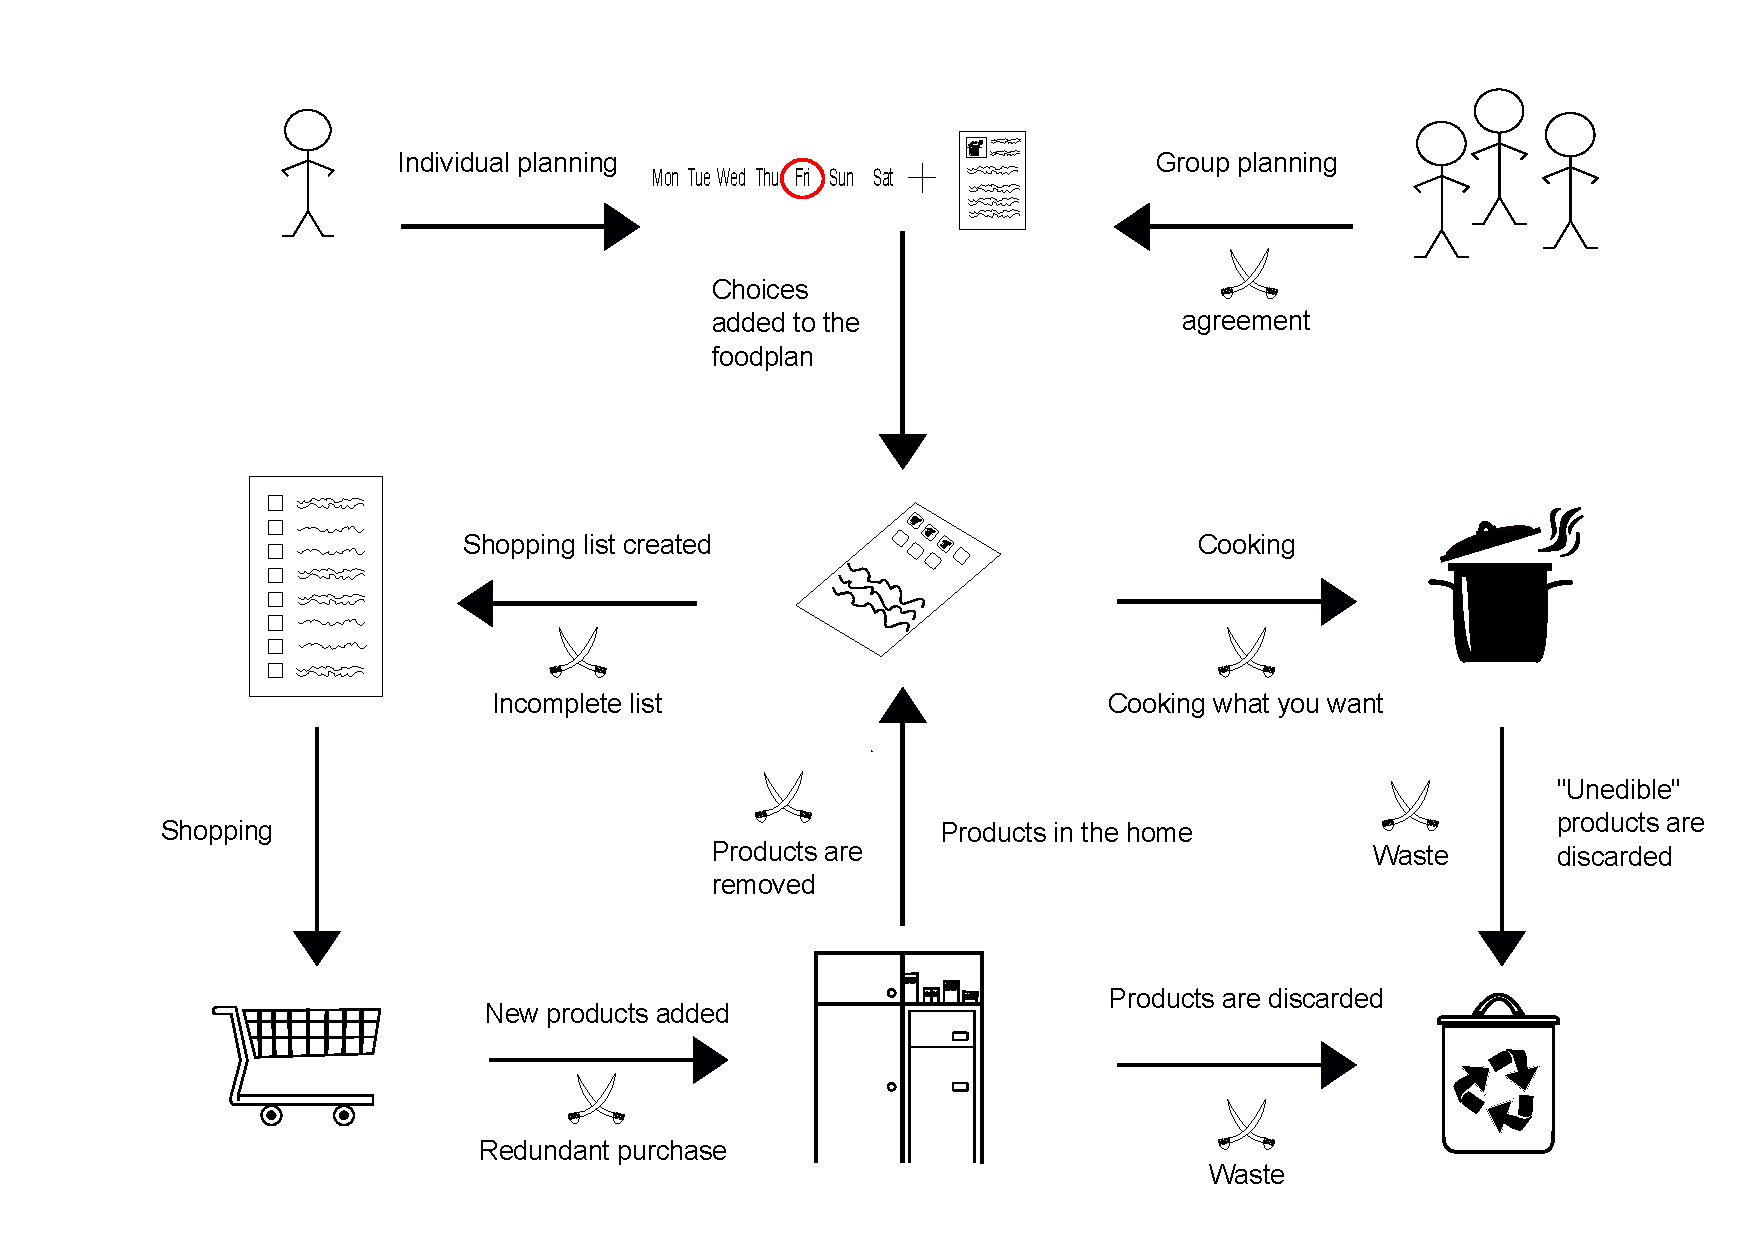
\includegraphics[width=1.00\textwidth]{Grafik/FoodPlanner/InkscapeTegninger/RigtBilledeUpdated.pdf}
	\caption{A rich picture of the user's situation from the viewers position}
	\label{RigtBillede}
\end{figure}
\fxnote{resize elementer så de er lige store + kosmetiske fejl}
\textbf{Units} includes people, physical objects, organizations and roles.
\begin{itemize}
  \item On the top line the stick man symbol is used to represent a user and to the top right there is the group of users symbol. 
  \item On the middle line is the overview of the food plan symbol and shopping list symbol which is used to depict the users overview of the two units. 
  \item On the bottom line is the inventory symbol used to depict the household's storage of food products and the trashcan symbol.    
\end{itemize}
\textbf{Processes} includes different categories such as work and production, planning and control and information treatment. In \Cref{RigtBillede} all of the arrows between the symbols signifies different processes.
\begin{itemize}
\item On the top line there are two arrows pointing into the schedule meal symbol signifying the process of choosing a specific day and a associated recipe. The choice is then added to the food plan showed by the vertical arrow pointing down to the overview of the food plan symbol. 

\item On the middle line there are two horizontal arrows. The arrow pointing to the left shows how a shopping list is created using data from the food plan. The arrow pointing to the right signifies the cooking work process. Below the middle line there are three vertical arrows. The arrow on the left pointing downwards shows the shopping process, the middle arrow pointing upwards signifies that the food plan is affected by what products that are in storage and the right arrow pointing downwards shows that products can be discarded when the user is cooking. 

\item On the bottom line there are two arrows pointing to the right. The left arrow signifies that products are added to the inventory after they are bought. The right arrow signifies that products can be discarded from the inventory.            
\end{itemize}
\textbf{Problems} describes the conflicts, contradictions and discrepancies in the situation.
\begin{itemize}
\item On the top line there is a conflict under the group planning process. This conflict is named synchronizing and happens when multiple users are scheduling meals. 

\item On the middle line there are two conflicts. The left one is named incomplete list and happens if the user does not have a complete list over the items that are needed in the food plan. The right conflict is named cooking what you want and describes that users can cook meals that are not on their food plan. Next there are the products removed conflict which happens when a user physically removes a product from the inventory. Next to this conflict we have the waste conflict which happens when food is thrown out during cooking.  

\item On the bottom line there are two more conflicts. The left one named redundant purchases, happens when the user buys larger quantities of food than the shopping list advises. The other conflict is called waste and happens when food from the inventory is thrown out just as the other waste conflict described just before.           
\end{itemize}
\textbf{Situations explained}

The starting points in \Cref{RigtBillede} are on the top line where a user or a group of users plan a meal by choosing a day and a recipe. In this process a conflict can occur when multiple users have to agree on a certain day and a specific meal. When a meal is planned it gets added to the food plan which can contain one or more meals. It is now possible for the user to get an overview of their meal plan and take actions to follow the plan. The first action might be writing a shopping list of what they need. In this process a conflict can occur if the user is not certain on which food products and how much that is needed, resulting in an incomplete shopping list. The user will now take their shopping list and go shopping for the specified items. 

The food products are then added to the inventory. During this process a conflict can occur if the user buys larger quantities of products than what was written in the shopping list. The products in the users inventory has an effect on the food plan. This effect is seen when the shopping list is written because products that are in the home should not be on the list. A conflict can occur if needed products are removed and not added to the shopping list. 

Another process that starts from the overview of the food plan is cooking. This process can create a conflict if the user cooks a meal that is not planned. This results in products that have been bought for the planned meal is not used and might not get used before they are thrown out. Food products can be thrown out from the inventory and from the cooking process. This can result in food waste if the discarded products could have been used in a future meal.      
\fxnote{\Cref{RigtBillede} can also be divided into different context areas. The areas represent contexts in which different symbols and processes are performed most often. The contexts are in the home and out of the home.}
   


      
\chapter{System Choice}
In this chapter the three sub activities Situation, Ideas and System definition when defining the system will be described and the system defined.
To describe the system choice we will be using systems development where system choice will be described this way situation, ideas and systems.

\fxnote{Brug slides fra lektion 3 SU for at skrive introer til afsnit.}
\section{Situation}
\Cref{RigtBillede} shows a Rich picture. This rich picture gives an overview of the users situation from the viewers position.
The symbols represent different units, processes and problems.
To begin with there will be looked upon the symbols and they will be explained. Afterwards the situation will be explained in depth.

  \begin{figure}[H]
	\centering
	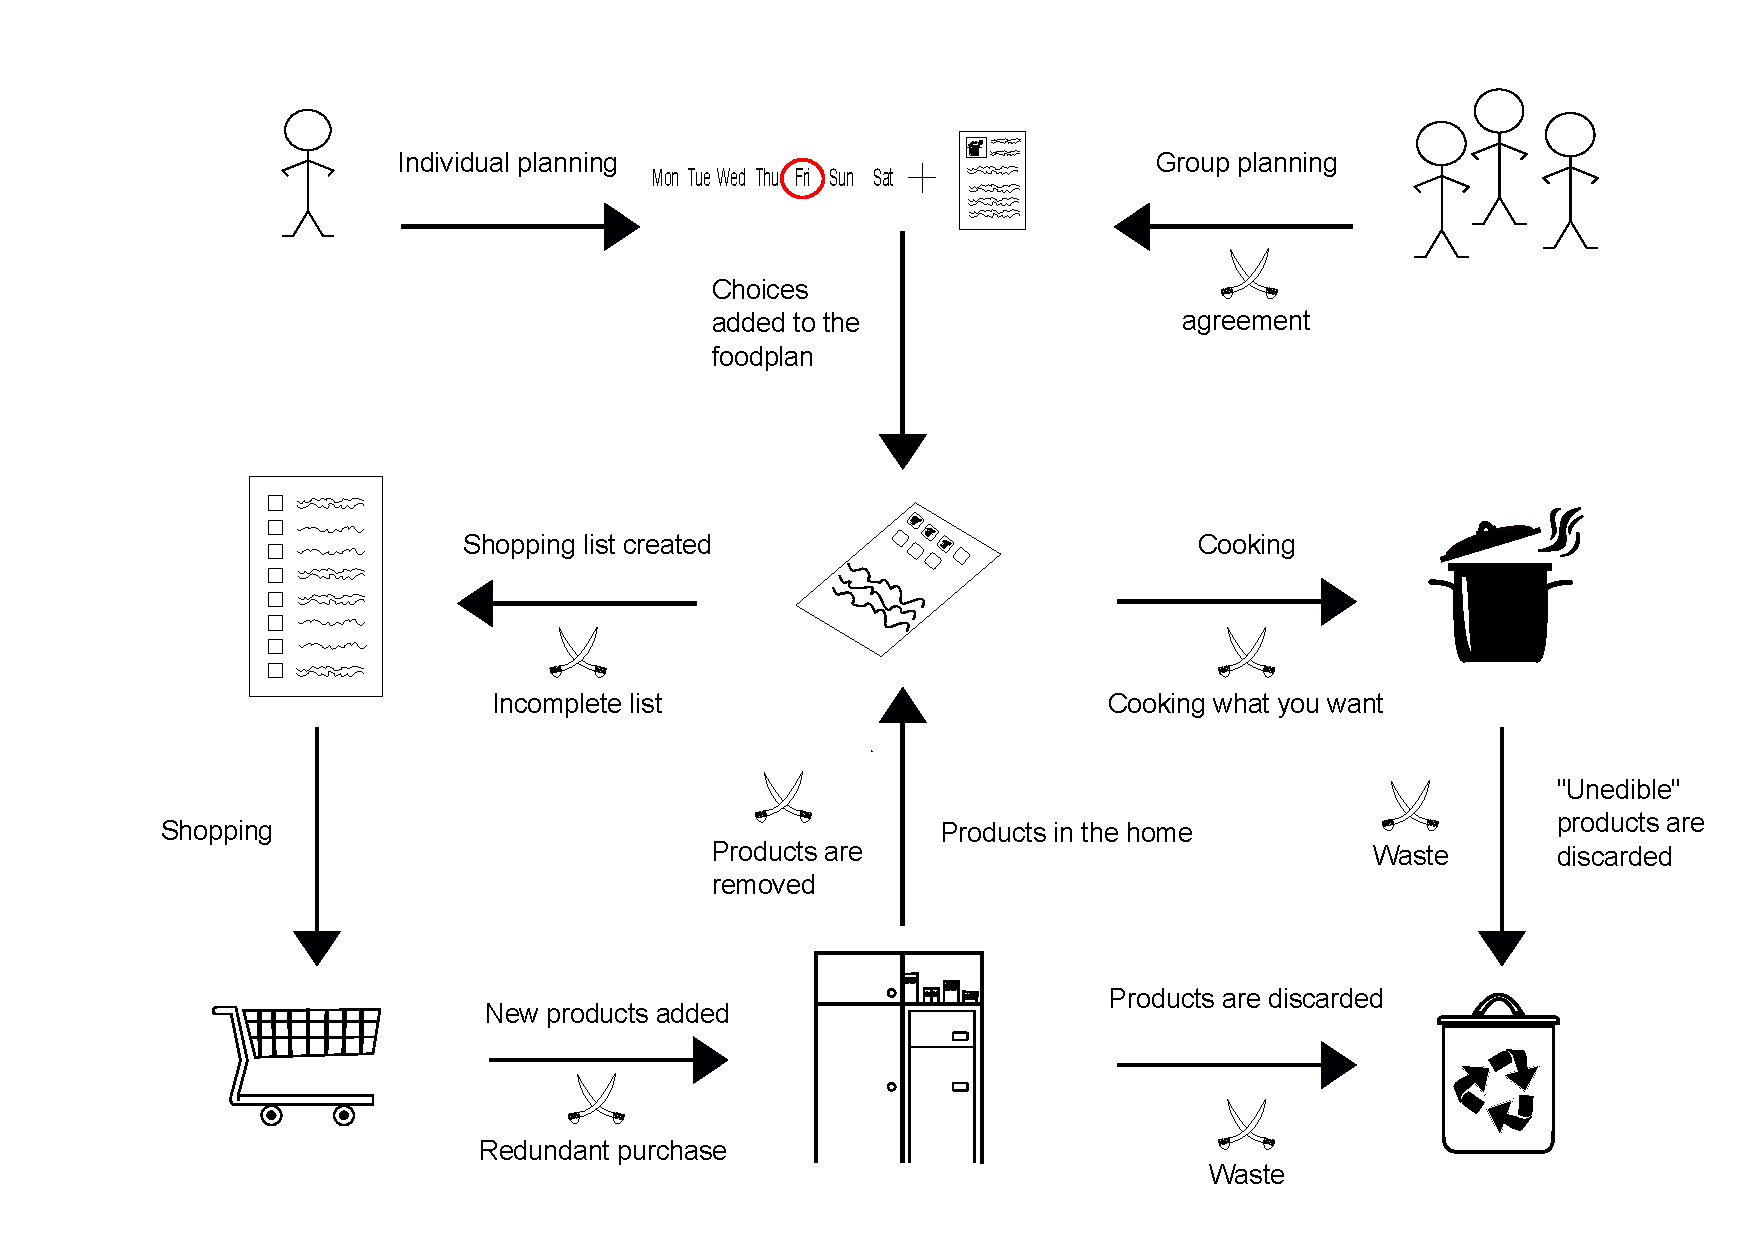
\includegraphics[width=1.00\textwidth]{Grafik/FoodPlanner/InkscapeTegninger/RigtBilledeUpdated.pdf}
	\caption{A rich picture of the user's situation from the viewers position}
	\label{RigtBillede}
\end{figure}
\fxnote{resize elementer så de er lige store + kosmetiske fejl}
\textbf{Units} includes people, physical objects, organizations and roles.
\begin{itemize}
  \item On the top line the stick man symbol is used to represent a user and to the top right there is the group of users symbol. 
  \item On the middle line is the overview of the food plan symbol and shopping list symbol which is used to depict the users overview of the two units. 
  \item On the bottom line is the inventory symbol used to depict the household's storage of food products and the trashcan symbol.    
\end{itemize}
\textbf{Processes} includes different categories such as work and production, planning and control and information treatment. In \Cref{RigtBillede} all of the arrows between the symbols signifies different processes.
\begin{itemize}
\item On the top line there are two arrows pointing into the schedule meal symbol signifying the process of choosing a specific day and a associated recipe. The choice is then added to the food plan showed by the vertical arrow pointing down to the overview of the food plan symbol. 

\item On the middle line there are two horizontal arrows. The arrow pointing to the left shows how a shopping list is created using data from the food plan. The arrow pointing to the right signifies the cooking work process. Below the middle line there are three vertical arrows. The arrow on the left pointing downwards shows the shopping process, the middle arrow pointing upwards signifies that the food plan is affected by what products that are in storage and the right arrow pointing downwards shows that products can be discarded when the user is cooking. 

\item On the bottom line there are two arrows pointing to the right. The left arrow signifies that products are added to the inventory after they are bought. The right arrow signifies that products can be discarded from the inventory.            
\end{itemize}
\textbf{Problems} describes the conflicts, contradictions and discrepancies in the situation.
\begin{itemize}
\item On the top line there is a conflict under the group planning process. This conflict is named synchronizing and happens when multiple users are scheduling meals. 

\item On the middle line there are two conflicts. The left one is named incomplete list and happens if the user does not have a complete list over the items that are needed in the food plan. The right conflict is named cooking what you want and describes that users can cook meals that are not on their food plan. Next there are the products removed conflict which happens when a user physically removes a product from the inventory. Next to this conflict we have the waste conflict which happens when food is thrown out during cooking.  

\item On the bottom line there are two more conflicts. The left one named redundant purchases, happens when the user buys larger quantities of food than the shopping list advises. The other conflict is called waste and happens when food from the inventory is thrown out just as the other waste conflict described just before.           
\end{itemize}
\textbf{Situations explained}

The starting points in \Cref{RigtBillede} are on the top line where a user or a group of users plan a meal by choosing a day and a recipe. In this process a conflict can occur when multiple users have to agree on a certain day and a specific meal. When a meal is planned it gets added to the food plan which can contain one or more meals. It is now possible for the user to get an overview of their meal plan and take actions to follow the plan. The first action might be writing a shopping list of what they need. In this process a conflict can occur if the user is not certain on which food products and how much that is needed, resulting in an incomplete shopping list. The user will now take their shopping list and go shopping for the specified items. 

The food products are then added to the inventory. During this process a conflict can occur if the user buys larger quantities of products than what was written in the shopping list. The products in the users inventory has an effect on the food plan. This effect is seen when the shopping list is written because products that are in the home should not be on the list. A conflict can occur if needed products are removed and not added to the shopping list. 

Another process that starts from the overview of the food plan is cooking. This process can create a conflict if the user cooks a meal that is not planned. This results in products that have been bought for the planned meal is not used and might not get used before they are thrown out. Food products can be thrown out from the inventory and from the cooking process. This can result in food waste if the discarded products could have been used in a future meal.      
\fxnote{\Cref{RigtBillede} can also be divided into different context areas. The areas represent contexts in which different symbols and processes are performed most often. The contexts are in the home and out of the home.}
   


      

\section{Ideas}
\section{Exemplars}
In this section, the current IT-systems will be described and what other systems that can be used to plan what food to eat. We will find ideas from the existing systems and put them into the context of our program. \fxnote{CHS: Still don't know how to incorporate metaphors}

\subsection{Food Planner}
one technology that are currently being used to make a food plan is a mobile application called \textit{Food Planner}.
In this application the users can plan meals ahead of time, lookup recipes, look at what groceries that needs to be bought,
list what the user have in the fridge so the grocery list appends to the items in the fridge and more\fxnote{I cannot understand the last sentence..}. In the following we look at the application, to find ideas which will be good in the context of our program.\fxnote{CHS: thinks this sentence is poorly written..}

\begin{figure}[H]
    \centering
    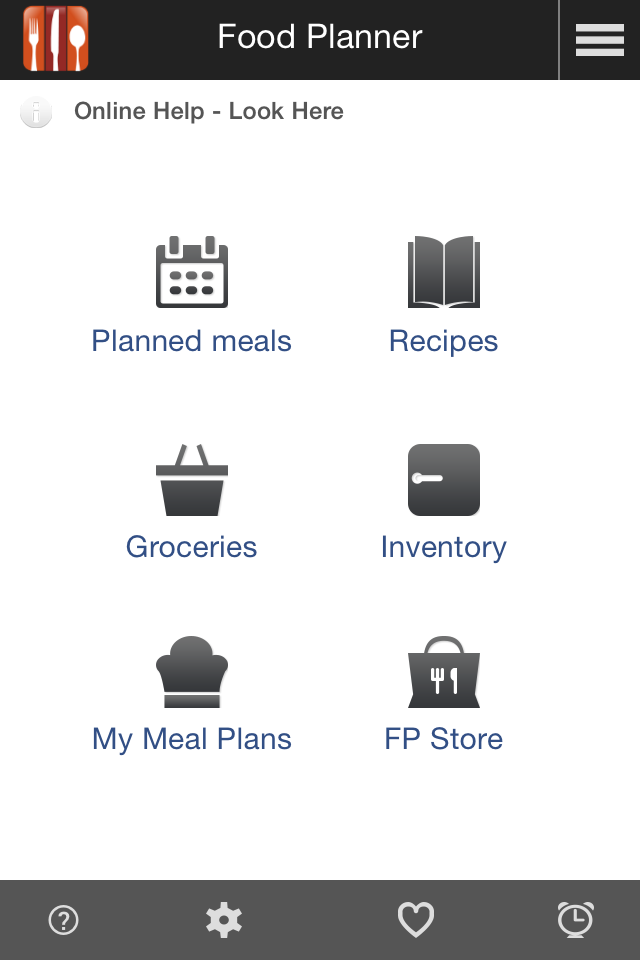
\includegraphics[width=0.5\textwidth]{Grafik/FoodPlanner/index}
    \caption{An image displaying the index of the application Food Planner}
    \label{FoodPlannerIndex}
\end{figure}
\begin{itemize}
  \item[Inventory:] Each product can be added separately, and the application can be used to keep track on the amount
  \item[Recipes:] Custom recipes can be created through the application, or they can be found/bought in the application store, or the internet, either by a Google search, or following a link directly to known websites, with recipes.
  \item[My meal plans:] this menu can keep track of meal planes, that has been added to the application.
  \item[Planned meals:] In this menu The upcoming days can be planed, with multiple recipes each day, either by adding them manually, or by adding a meal plan from \textit{My meal plans}. Missing groceries for a desired  number of days ahead, can then automatically be added to a \textit{Grocery menu}.
  \item[Registering:] By registering with an e-mail and a password, the application allows the user to back up the information, synchronizing with other devises and sharing is also enabled.
  \item[Grocery menu:] Here groceries that needs to be bought can be added, either automatically from \textit{My meal plan}, or added manually. If an item does not exist in the program, it can be added using a bar-code scanner.
\end{itemize}
\fxnote{Kan filføle flere billeder af FoodPlanner appen og uddube dem.}

\subsection{Website}
Another alternative could be a tool found on the website madplanuge.dk\cite{madSpild_madPlanUge}. This tool is a basic foodplanner, where the foodplan can be planned one week ahead, but the users storage is taken into consideration.

When the user enters the website the user can either choose between 20 random recipes or search for something the user would like to eat.
Then the user can choose up to 3 recipes for each of the days so the user can plan breakfast, lunch and dinner for each specific day.
After the food plan has been selected, the user can then get a shopping list of all the needed items.
If the user creates a user on the site, the user will be able to save, and favorite different recipes.
If the user finds a recipe with some ingredients who the user likes, would the user be able to get more recipes based upon those ingredients.

\begin{figure}[H]
    \centering
    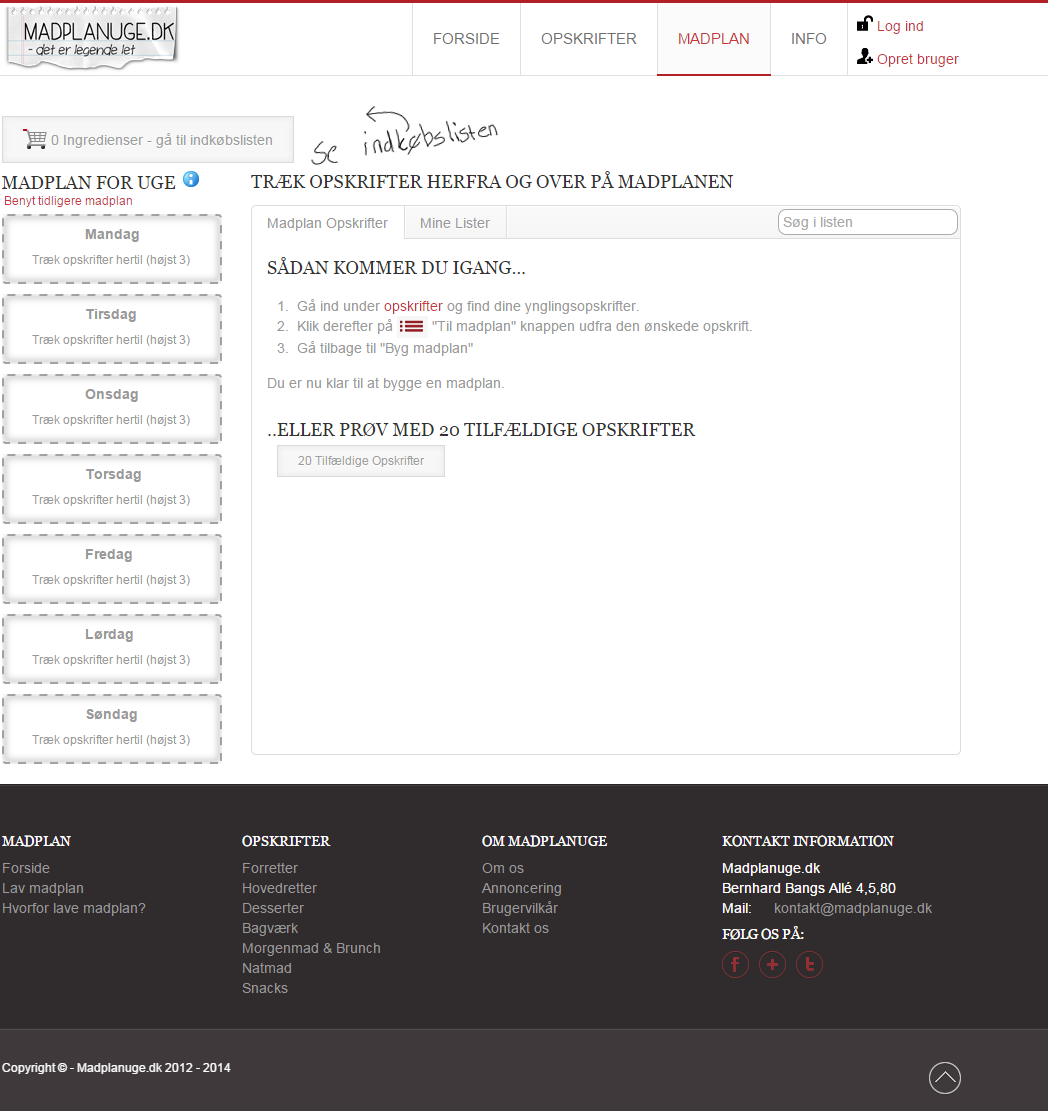
\includegraphics[width=0.5\textwidth]{Grafik/madplanuge}
    \caption{An image displaying the the website Madplan Uge}
    \label{MadPlanUge}
\end{figure}


\section{System}
\subsection{Definition (FACTOR)}
To formulate a system definition we used the FACTOR \cite{OOAD_BATOF} criteria to establish important parts of the system.

\begin{description}
	\item[Functionality] Help users organize a meal plan based on their preferences and inventory. Create/edit user, inventory and plan.
	\item[Application domain] Database responsible employees \fxnote{what is this (explain in definition below)}, Users planning meals.
	\item[Conditions] The system will be used by users with varying technical abilities and cooking experience.
	\item[Technology] Tablet, smartphone
	\item[Objects] Family member (user), inventory (groceries), recipe
	\item[Responsibility] An administrative/planning tool
\end{description}

\subsection{System Definition}
A system which primarily lets you plan your meals in advance based on what is in your inventory to assist the user and reduce food waste.
Secondarily the program will allow administration of a meal plan and inventory and incorporate functions to alter this plan and inventory by adding or removing recipes and groceries.
The system will be designed for tablets and smartphones, as these devices offers mobility and thereby available both in and out of the user's home.
\chapter{Problem Domain}
In this chapter the reality the user is going to see will be described. This reality is constructed of the areas which the system is going to administrate, monitor or control. Descriptions of classes, objects, structures and behaviours will be made throughout the chapter.


\section{Classes}\label{ClassesLabel}
In this section a list of classes will be presented. The classes described are those which have been chosen through a class candidate analysis.

\subsection{Physical}
\begin{itemize}
\item \textbf{Product:} This class is used to identify different ingredients for the recipes with information such as food type and expiration date. This class is essential for the program and will be used frequently.
\item \textbf{Recipe:} This class holds information about the ingredients and instructions on how to cook the meal.
\item \textbf{Scheduled Meal:} This class contains information about a recipe and when it is scheduled to be cooked.
\end{itemize}

\subsection{Persons}
\begin{itemize}
\item \textbf{User:} This class contains information about the preferences of a specific user, and will allow the solution to synchronise/share data with other users or devices.
\end{itemize}

\subsection{Places}
\begin{itemize}
\item \textbf{Shop:} This class holds information about the location of specific groceries and discounts.
\end{itemize}

\section{Events}
In this section a list of events will be presented. The events described are those which have been chosen through an event candidate analysis. The events and what trigger them are listed below.
\subsection{Consumption}
\begin{itemize}
\item \textbf{Product bought:} A shopping list have been completed. The items bought will be added to an inventory.
\item \textbf{Product removed:} A meal have been prepared and the product should be removed from the inventory, or have an subtraction from its original volume/quantity.
\item \textbf{Product expired:} When a product reaches its expiration date, it should be removed from the inventory and thrown out.
\end{itemize}

\subsection{Planning}
\begin{itemize}
    \item \textbf{Recipe scheduled:} When a recipe is scheduled for a date in the meal plan.
    \item \textbf{Recipe removed:} When the user removes a recipe which was scheduled for a date in the meal plan.
    \item \textbf{Shopping list item added:} When a recipe have been scheduled in the meal plan, missing ingredients from the inventory are added to the shopping list.
\end{itemize}

\subsection{Preferences/settings}
\begin{itemize}
\item \textbf{Preference changed:} When the user navigates to a settings menu to exclude products from the system, due to allergies, diets or preference.
\end{itemize}

\section{Event Table}
\Cref{tab:EventTable} shows an event table that have been constructed in order to get an overview of the relations between classes and events. The event table allows for a better judgement of which classes are relevant in the program. A plus (+) in the table indicates, that an event can occur zero or one time, whereas a star (*) indicates that an event can occur zero or more times.

\begin{table}[H]\centering
    \begin{tabular}{|r|c|c|c|c|}
        \hline
        ~                                      & Product & Recipe & User & Meal\\ \hline
        \textbf{Consumption}                   & ~       & ~      & ~    & ~   \\ 
		    Product added                          & +       & ~      & ~    & ~   \\ 
        Product removed                        & +       & ~      & ~    & ~   \\ 
        Product expired                        & *       & ~      & ~    & ~   \\ 
        Product unexpired                      & *       & ~      & ~    & ~   \\ 
        Product quantity changed               & *       & ~      & ~    & ~   \\ 
        Product expiration changed             & *       & ~      & ~    & ~   \\ 
        \textbf{Planning}                      & ~       & ~      & ~    & ~   \\ 
        Shopping list item added               & +       & ~      & ~    & ~   \\ 
        Meal added                             & ~       & +      & ~    & +   \\ 
        Meal removed                           & ~       & +      & ~    & +   \\ 
        Meal rescheduled                       & ~       & +      & ~    & +   \\ 
        Meal participants changed              & ~       & ~      & ~    & *   \\ 
        Meal Date changed                      & ~       & ~      & ~    & *   \\ 
        \textbf{Other}                         & ~       & ~      & ~    & ~   \\ 
        Preference changed                     & ~       & ~      & *    & ~   \\ 
		    Recipe found                           & ~       & *      & ~    & ~   \\ 
		\hline    
    \end{tabular}
    \caption{An event table for the program} 
    \label{tab:EventTable}
\end{table}
\section{Event Traces} \label{EventTraces}
This section will present a statemachine diagram for each class. Each statemachine diagram is the result of examining each class, with a focus on identifying the different states of the class' objects and the events, which effects the objects and changes their state. An event can happen without changing the state of the class e.g. on \cref{MealClass} the \textit{Change scale} event will not lead to a new state for the meal class object.  

Each class examination first shows a few of the event traces that were formulated for the specific class. The relationship between the classes and events are described in \cref{tab:EventTable}. The event traces will be used to model the statemachine diagram for the specific class. The event traces and statemachine diagrams are created to get a better understanding of the dynamic in the problem domain. It is possible to use the event definitions in \cref{EventsSection} for a better understanding of each event, if the event behaviour is not clear from the event name.   

\subsection{Food Class}
Some of the event traces used to understand the behaviour of this class are:
\begin{itemize}
	\item \textit{Added} -> \textit{Expired} -> \textit{Quantity changed} -> \textit{Removed}.
	\item \textit{Added} -> \textit{Quantity changed} -> \textit{Expired} -> \textit{Quantity changed} -> \textit{Unexpired} -> \textit{Removed}.
	\item \textit{Shopping list item added} -> \textit{Added} -> \textit{Expired} -> \textit{Removed}.
	\item \textit{Shopping list item added} -> \textit{Shopping list item removed}.
\end{itemize}

This class also has some event traces which are not legal e.g. 
\textit{Shopping list item added} -> \textit{Expired}.

\begin{figure}[tbhp]
	\centering
	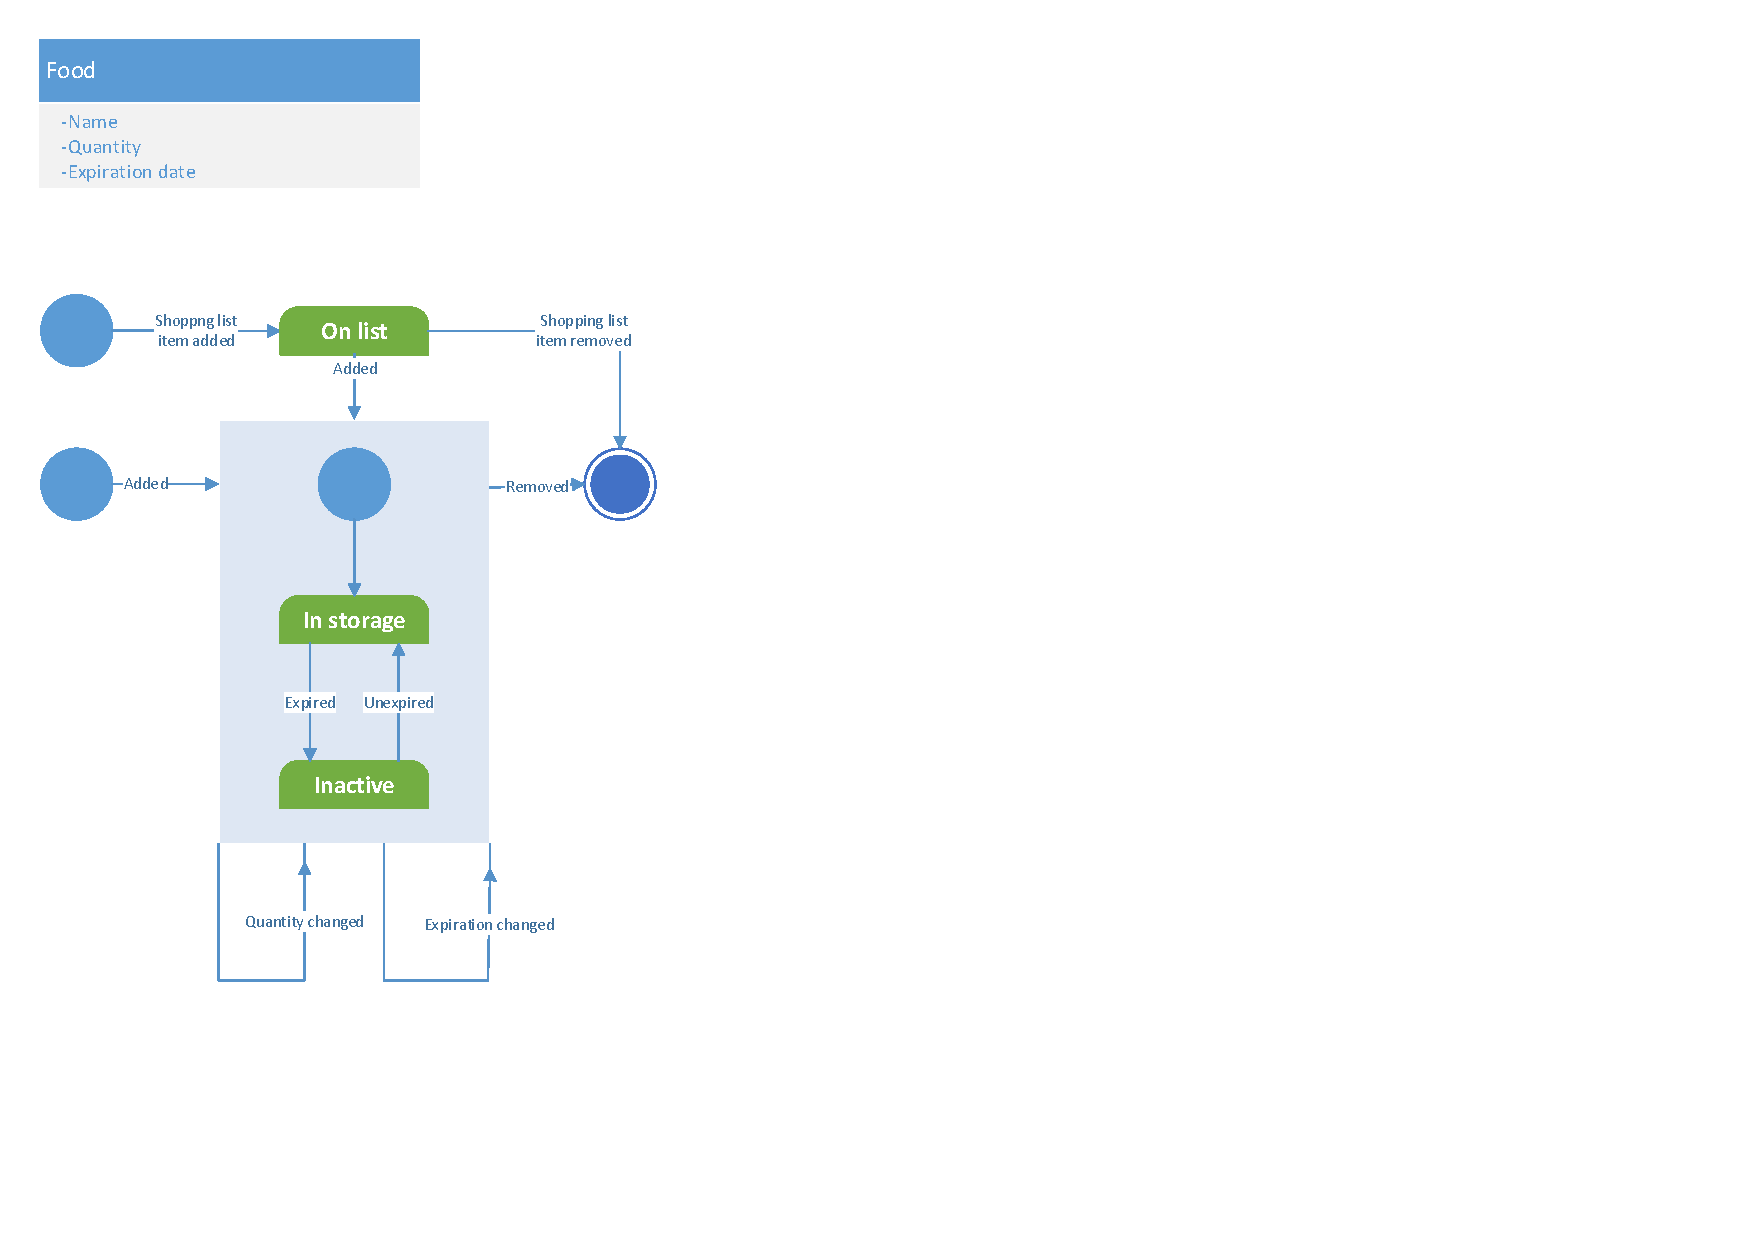
\includegraphics[clip=true, trim=0.5cm 4cm 18.5cm 0.5cm,  ]{Grafik/FoodPlanner/Food.pdf}
	\caption{Statemachine diagram for the Food class.} \label{FoodClass}
\end{figure}
An object of this class can be instantiated when the user either adds a shopping list item or adds a food item directly to their inventory. The two starting events for this class are therefore \textit{Shopping list item added} and \textit{Added}. The two start events sets the object's state to either \textit{On list} or \textit{In storage}. The On list state can be changed by the Add event, which sets the state to In storage, or by the \textit{Shopping list item removed} event, which terminates the object. The object can also have the state \textit{Inactive}, which can be set by the \textit{Expired} event and reset to the In storage state by the \textit{Unexpired} event. It is possible for an object in both the In storage and Inactive state to be effected by the \textit{Quantity changed} and \textit{Expiration changed} event, without changing the object's state. These two events can be iterated throughout an object's lifetime. The object can also be terminated from the In storage and Inactive state, by the \textit{Removed} event.   

\subsection{Meal Class}
Some of the event traces used to understand this class are:
\begin{itemize}
	\item \textit{Meal added} -> \textit{Change scale} -> \textit{Meal prepared}.
	\item \textit{Meal added} -> \textit{Change date} -> \textit{Meal prepared}.
	\item \textit{Meal added} -> \textit{Day passed} ->\textit{ Reschedule meal} -> \textit{Meal prepared}.
	\item \textit{Meal added} -> \textit{Change scale} -> \textit{Change date} -> \textit{Change scale} -> \textit{Meal prepared}.
\end{itemize}

An example of event traces that are not legal for this class are: \textit{Meal added} -> \textit{Day passed} -> \textit{Change Scale}.

\begin{figure}[H]
	\centering
	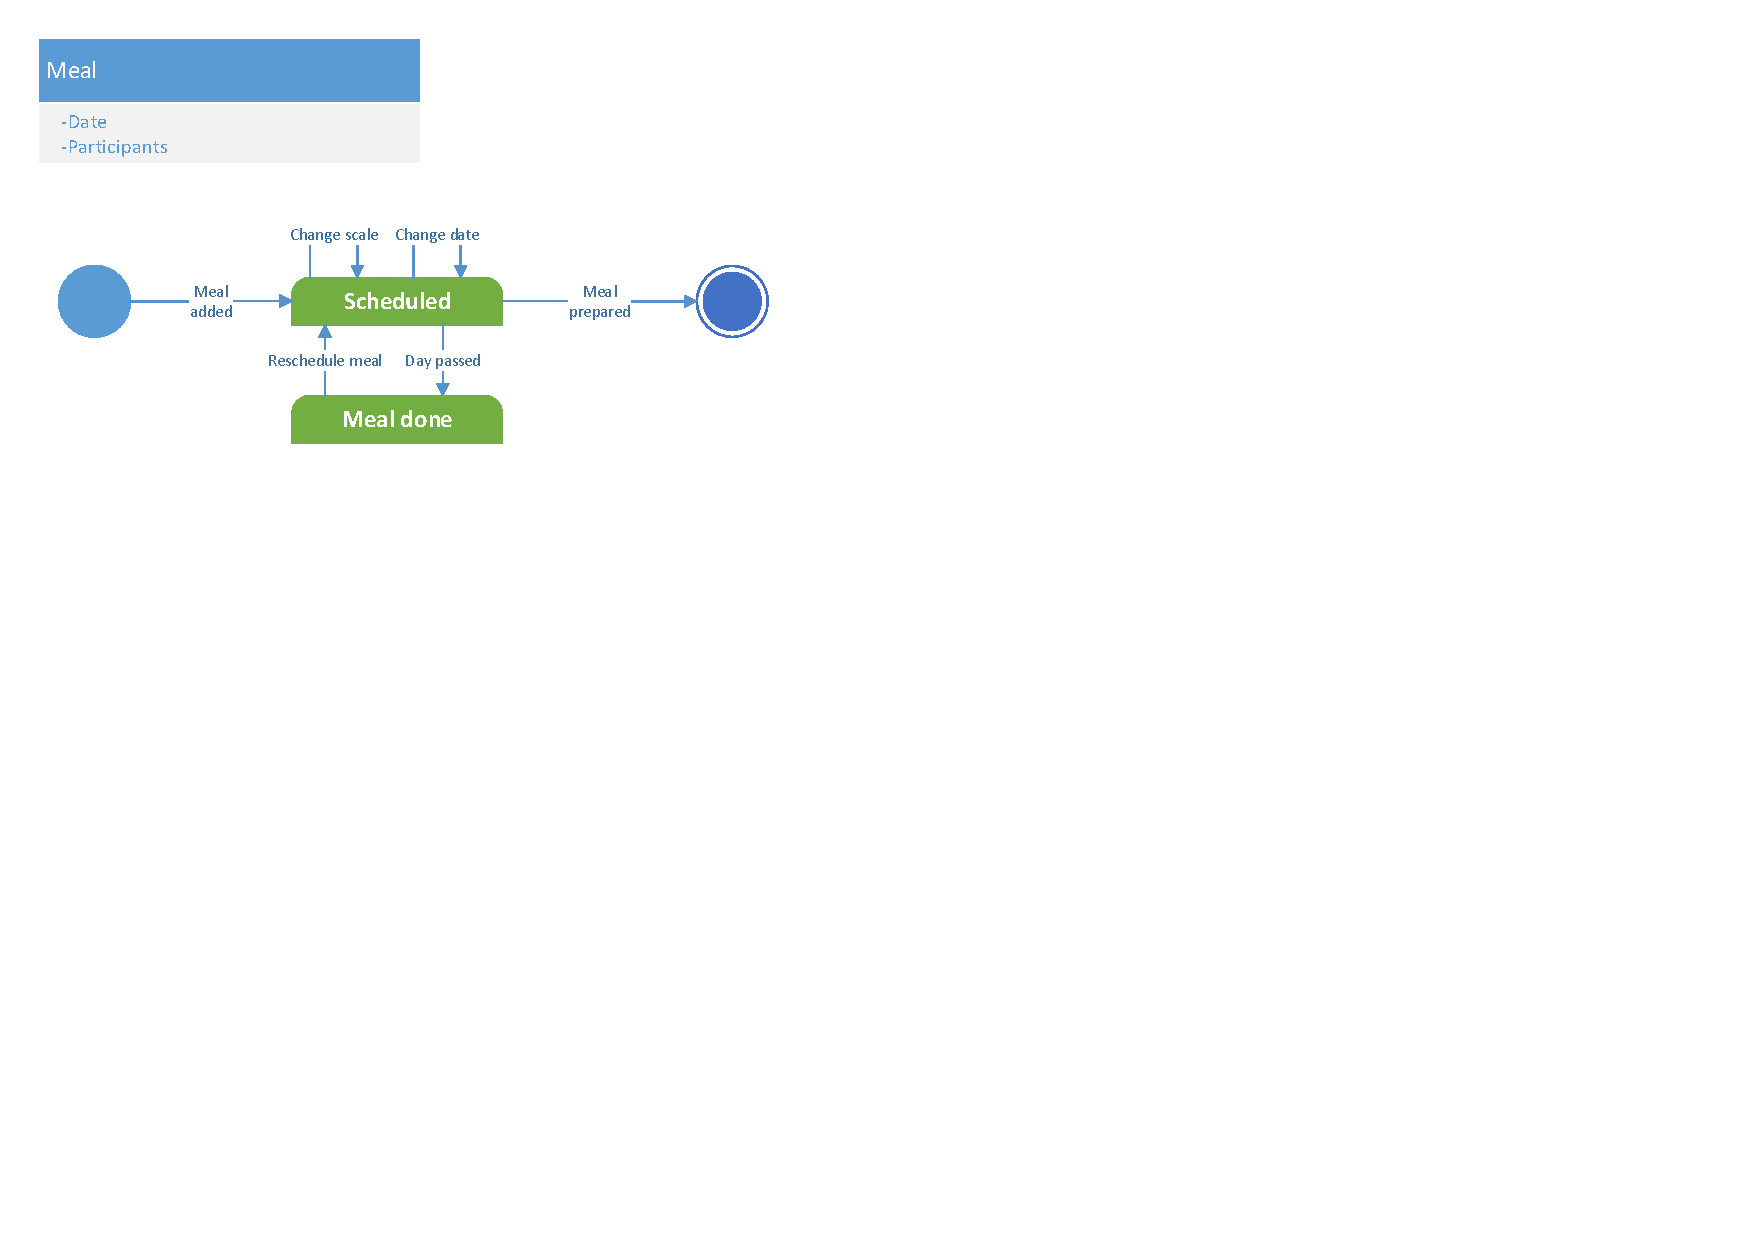
\includegraphics[clip=true, trim=0.5cm 13cm 16.5cm 0.5cm]{Grafik/FoodPlanner/Meal.pdf}
	\caption{Statemachine diagram for the Meal class.} \label{MealClass}
\end{figure}

An object of the meal class can be instantiated by the \textit{Meal added} event, and this sets the state of the object to \textit{Scheduled}. The events \textit{Change scale} and \textit{Change date} can be iterated throughout the object's lifetime, and does not change the state of the object. The object can also have the \textit{Meal done} state, which can be set by the \textit{Day passed} event and reset to the Scheduled state by the \textit{Reschedule meal} event. The object can only be terminated by the \textit{Meal prepared} event.

\subsection{User Class}
Some of the event traces used to better understand the events and flow of the User class are:

\begin{itemize}
	\item \textit{User registered} -> \textit{Preference added} -> \textit{Preference added} -> \textit{User deleted}.
	\item \textit{User registered} -> \textit{Preference added} -> \textit{Preference removed} -> \textit{User deleted}.
\end{itemize}

An event trace which is not legal for this class could be \textit{User registered} -> \textit{Preference removed} -> \textit{User deleted}.

\begin{figure}[H]
	\centering
	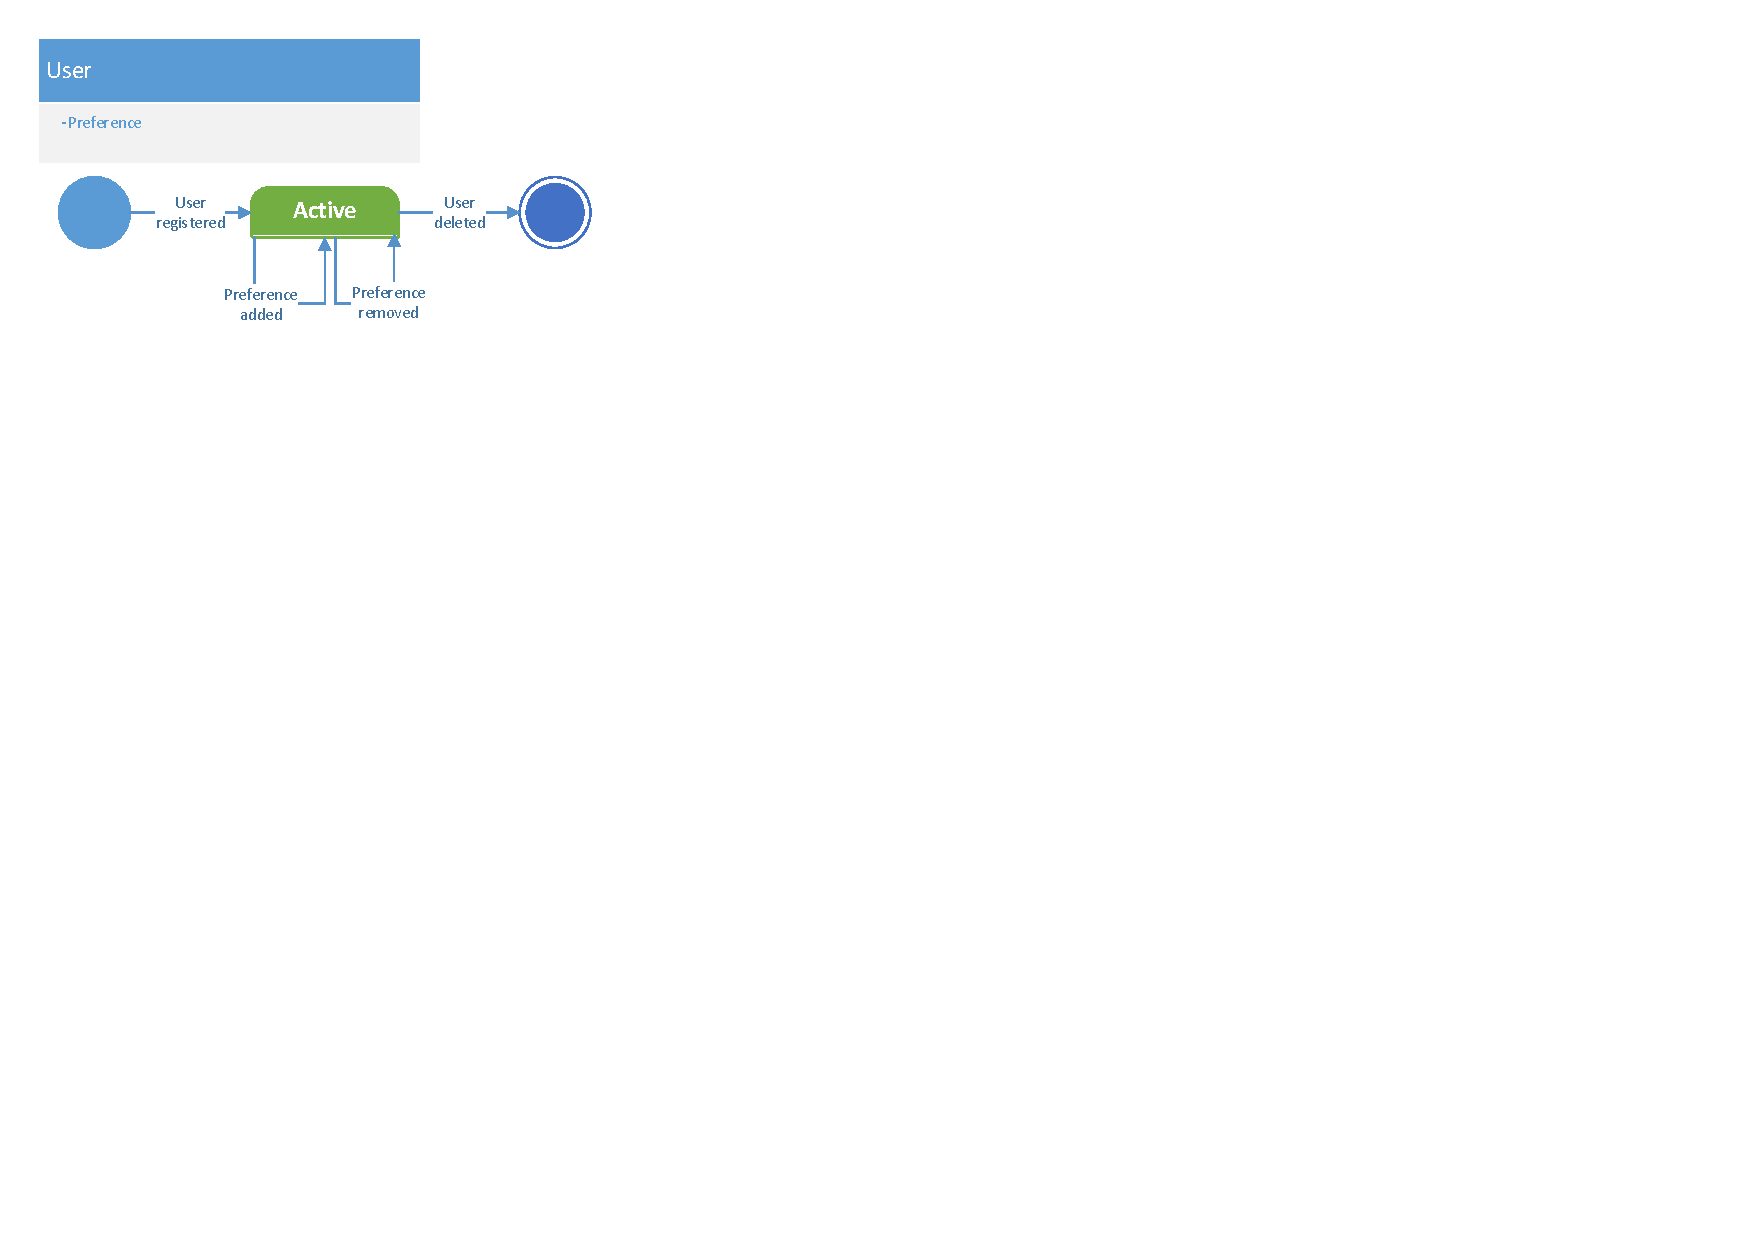
\includegraphics[clip=true, trim=0 14cm 5cm 0]{Grafik/FoodPlanner/UserSettings.pdf}
	\caption{Statemachine diagram for the User class.} \label{UserSettingsClass}
\end{figure}

This class can have an object instantiated by the \textit{User registration} event, and this event sets the object's state to \textit{Active}. From this state the \textit{Preference added} and \textit{Preference removed} event can be iterated throughout the object's lifetime. The object can only be terminated by the \textit{User deleted} event.


\subsection{Recipe Class}
Some of the event traces used to understand the Recipe class are:
\begin{itemize}
	\item \textit{Recipe added} -> \textit{Recipe removed}.
	\item \textit{Recipe added} -> \textit{Recipe found} -> \textit{Meal added} -> \textit{Meal removed}.
	\item \textit{Recipe added} -> \textit{Recipe found} -> \textit{Recipe found} -> \textit{Meal added} -> \textit{Meal removed}.
\end{itemize}

One of the event traces which are not legal for this class are:\textit{ Recipe added }-> \textit{Recipe found} - \textit{Meal removed}.

\begin{figure}[H]
	\centering
	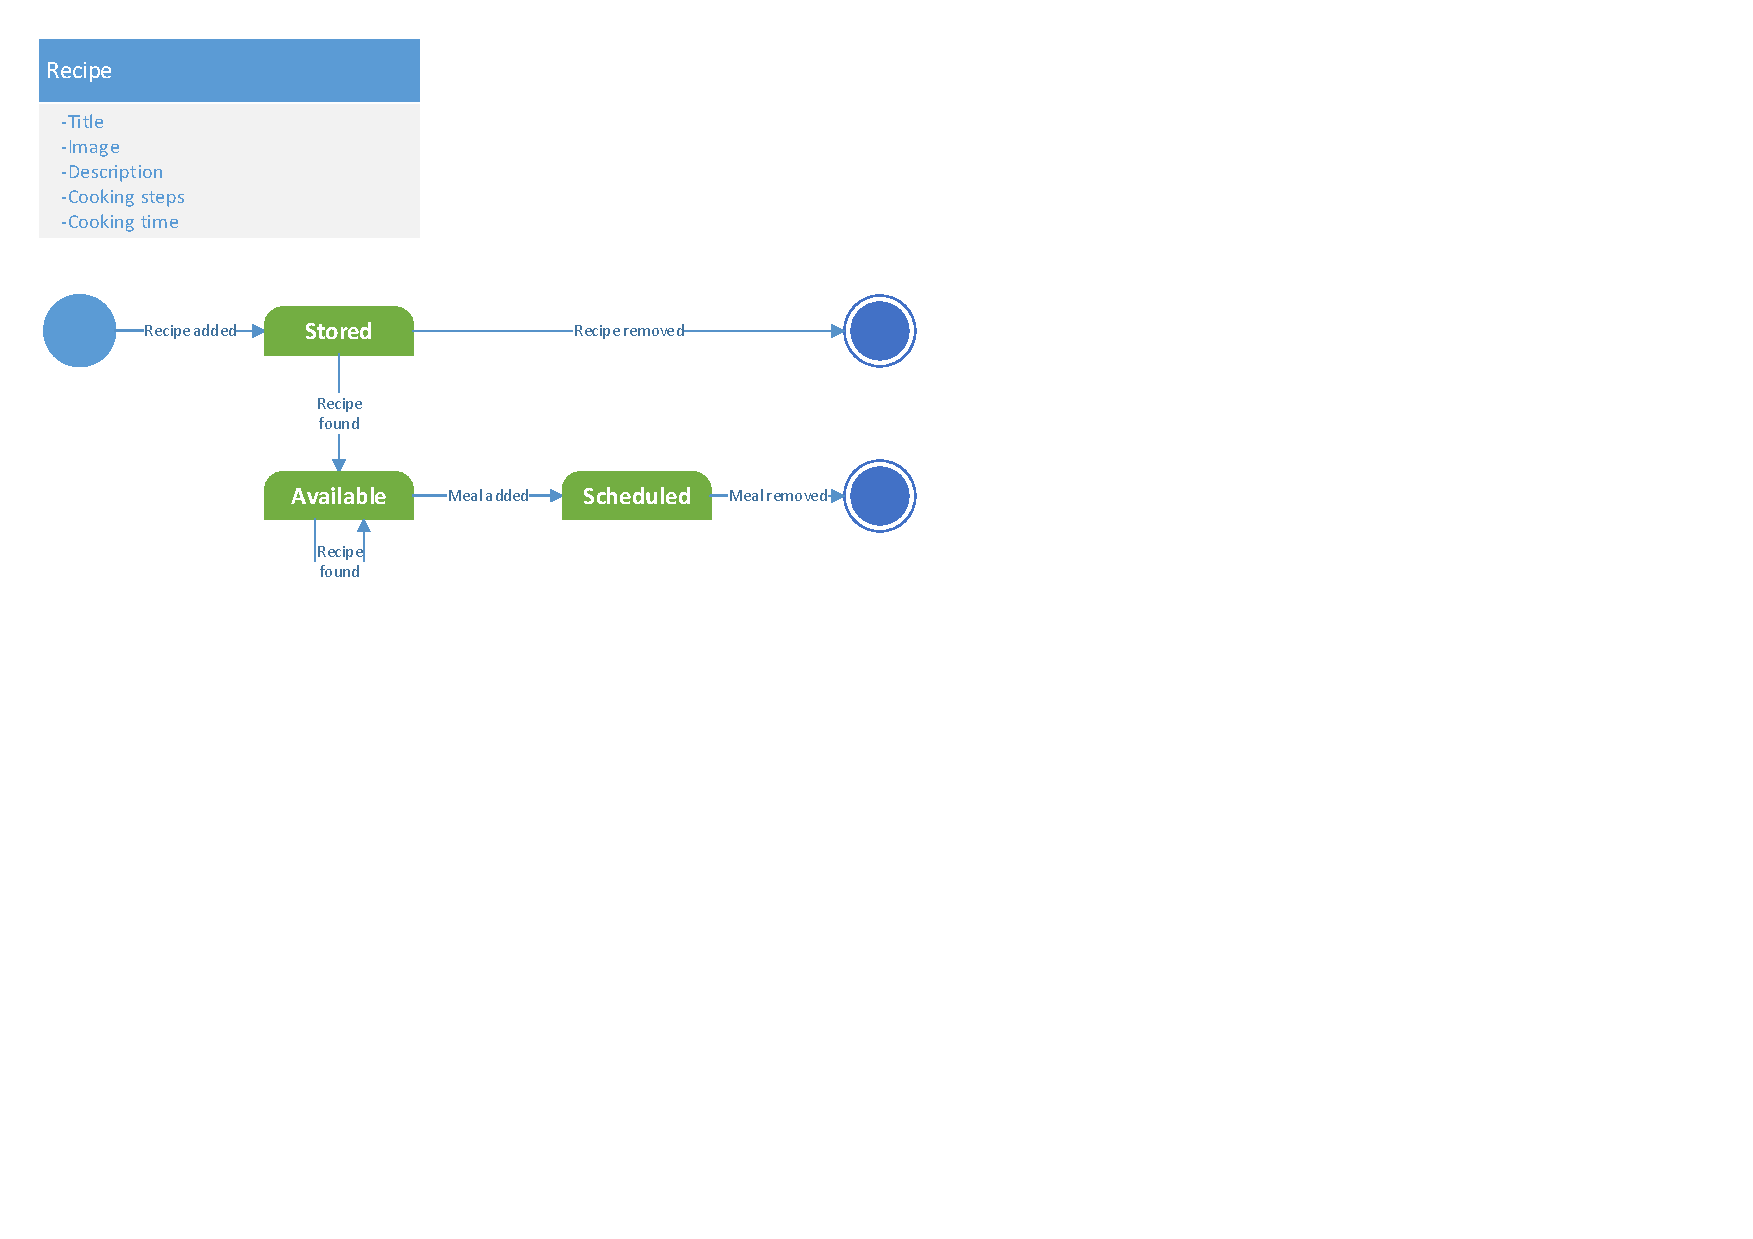
\includegraphics[clip=true, trim=0.5cm 11cm 14cm 0.5cm]{Grafik/FoodPlanner/Recipe.pdf}
	\caption{Statemachine diagram for the Recipe class.} \label{RecipeClass}
\end{figure}

An object of the Recipe class can only be instantiated by the \textit{Recipe added} event, and this event sets the state of the object to \textit{Stored}. From this state the \textit{Recipe removed} event can terminate the object. The \textit{Recipe found} event can change the object's state from Stored to \textit{Available}. The same event can also be iterated in this state, without changing the state. The \textit{Meal added} event can change the object's state to \textit{Scheduled}. From this state the \textit{Meal removed} event can terminate the object.

Anvendelsesområdet se side 296

\section{Usage}\label{Usage}
This section will describe the systems interaction with its surroundings. This will be done by making an actor specification and then presenting user pattern diagrams, which will be showcased in state machine diagrams.

\subsection{Actor specification}
\label{Actor_specification}
This system only contains one actor, which is the user of the system. The actor will be described by an actor specification.

\textbf{Objective:} A person who prepares meals, either for himself or for a household. The user's primary need is to plan his week in order to efficiently shop groceries and reduce food waste.

\textbf{Characteristic:} The system includes a user base of which the users have different needs and preferences.

\textbf{Example one:} User A is allergic to nuts and has to make meals which excludes these. When he is shopping he needs to look at the package info to make sure that the product does not contain traces of nuts.

\textbf{Example two:} User B is a young student who is in a relationship. He has a tight budget and a short time frame to shop in. The couple finds it difficult to sustain an overview of their shared storage of food. Therefore User B will sometimes buy products the couple do not need, for example, he might purchase milk even though they already have three litres stored. This will sometimes result in them not being able to use all the milk before it expires, which is bad for their shared budget and food waste.



\subsection{Use Cases}
The use cases shows how the actor interacts with the system to complete tasks. These interactions are shown in state machine diagrams. The diagrams show how the dynamic states can shift through interactions with the actor. Even though many of the details is excluded, it still gives an overview of the logic and flow behind the use cases.

The purpose of the diagram is to create an overview of the application domain's interactions with the system. This will be used to find requirements for the functions and user interface. There are three user pattern diagrams, each representing different areas of the system. The three diagrams showcase the user patterns in the:

\begin{itemize}
\item{Shopping list}
\item{Meal plan}
\item{Inventory}
\end{itemize}

When the user navigates the system, the user will undertake one of two roles. An administrative or a planning oriented role.
The option to go back or cancel have not been included in any of the diagrams, as their only contribution is to make the diagrams less readable and add redundant repetitions.

\Cref{Foodplan_Figure} shows the state machine diagram for planning meals. In this part of the system the user operates under the role of planning.

\begin{figure}[H]
	\centering
	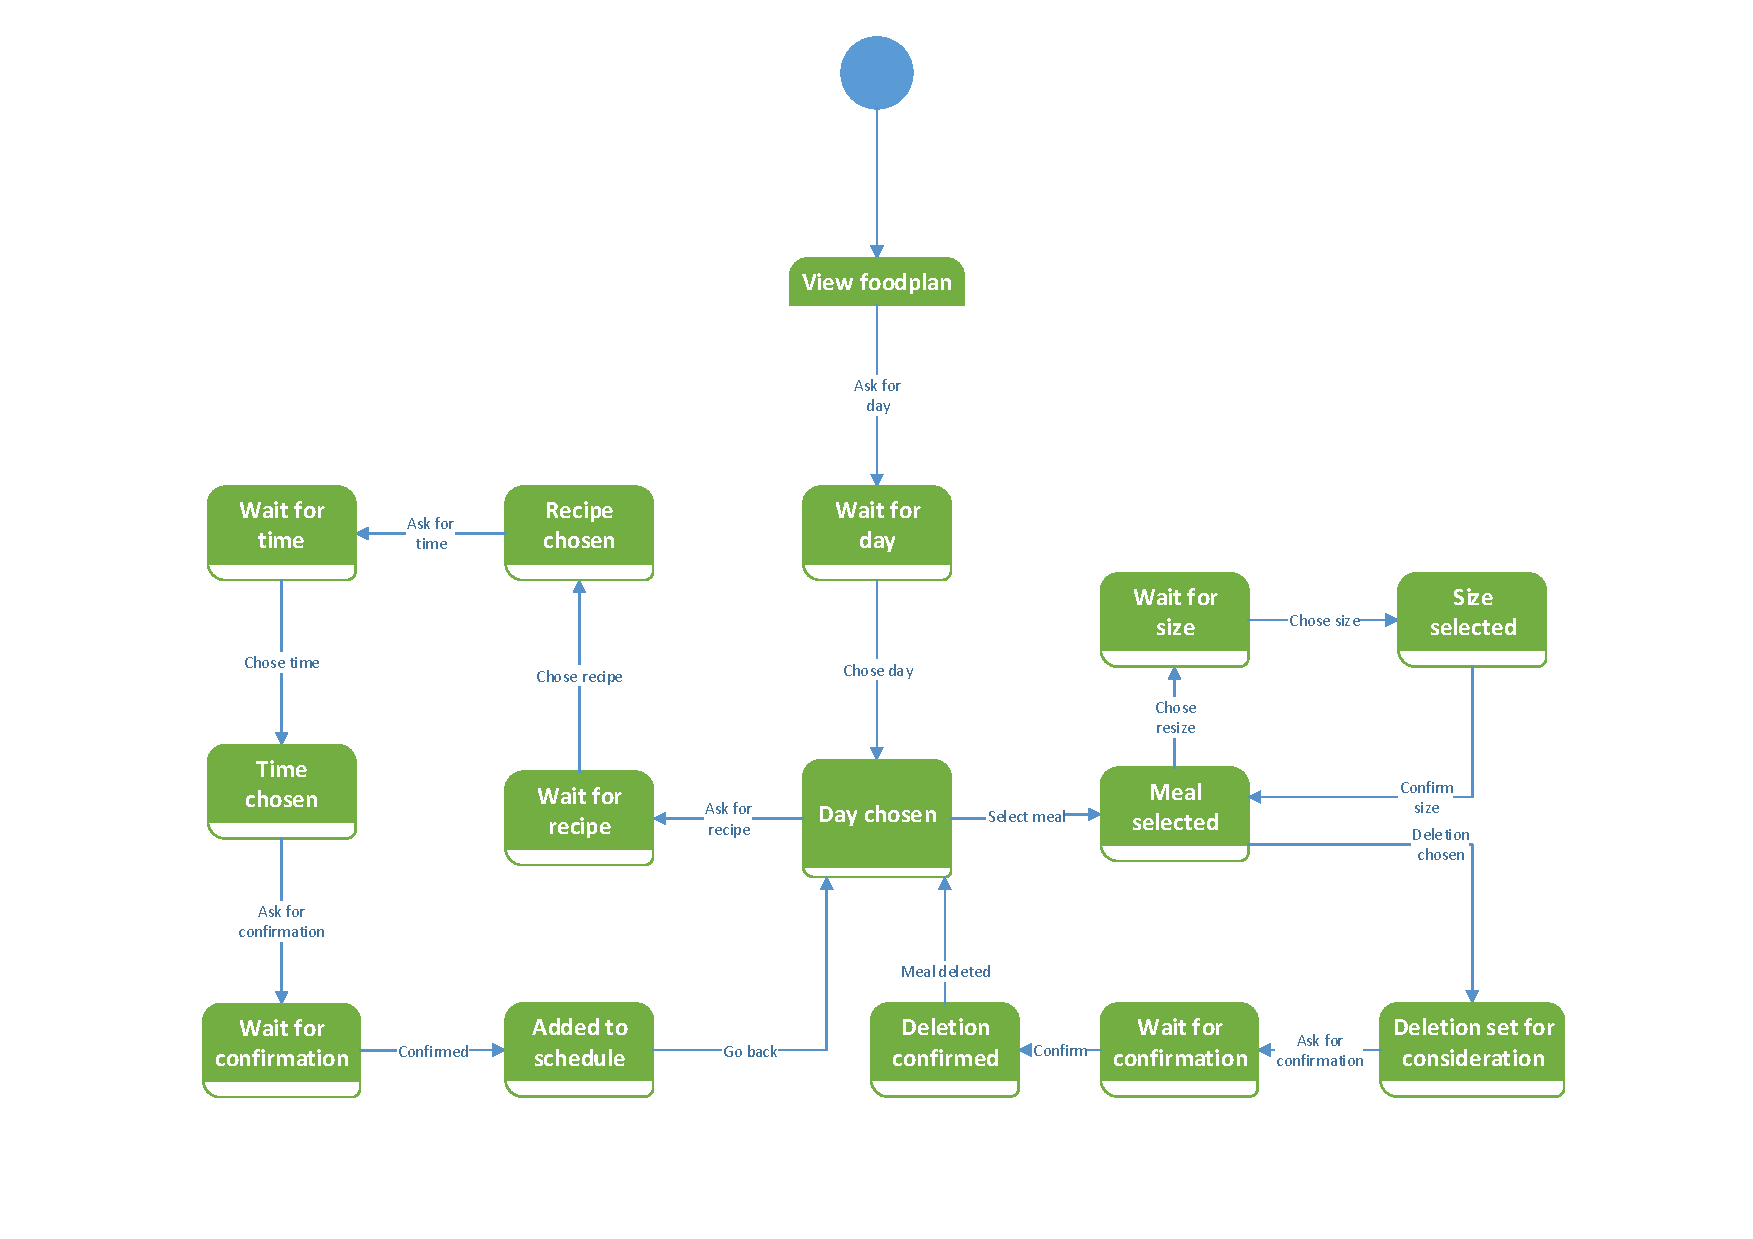
\includegraphics[width=1.0\textwidth]{ApplicationDomain/spViewFoodPlan.pdf} 
	\caption{State machine diagram for meal planning.}
	\label{Foodplan_Figure}
\end{figure}
When the user navigates to the meal plan part of the system, he will have to choose a day to view the meal plan for. From there the user can add a new meal to the plan or select an existing planned meal. If the user chooses to add a new meal, the system will ask for a recipe. The recipes the user can choose from varies depending on the user's preferences. If the user has chosen to avoid some products, recipes that contain those products will be excluded. When a recipe has been chosen, a time can be entered for when the meal should be prepared. After confirmation the meal will be added to the schedule.

The next two diagrams, \cref{Inventory_Figure} and \cref{spEditInventory}, are for the inventory. In this part of the system the user operates as an administrator.

\begin{figure}[H]
	\centering
	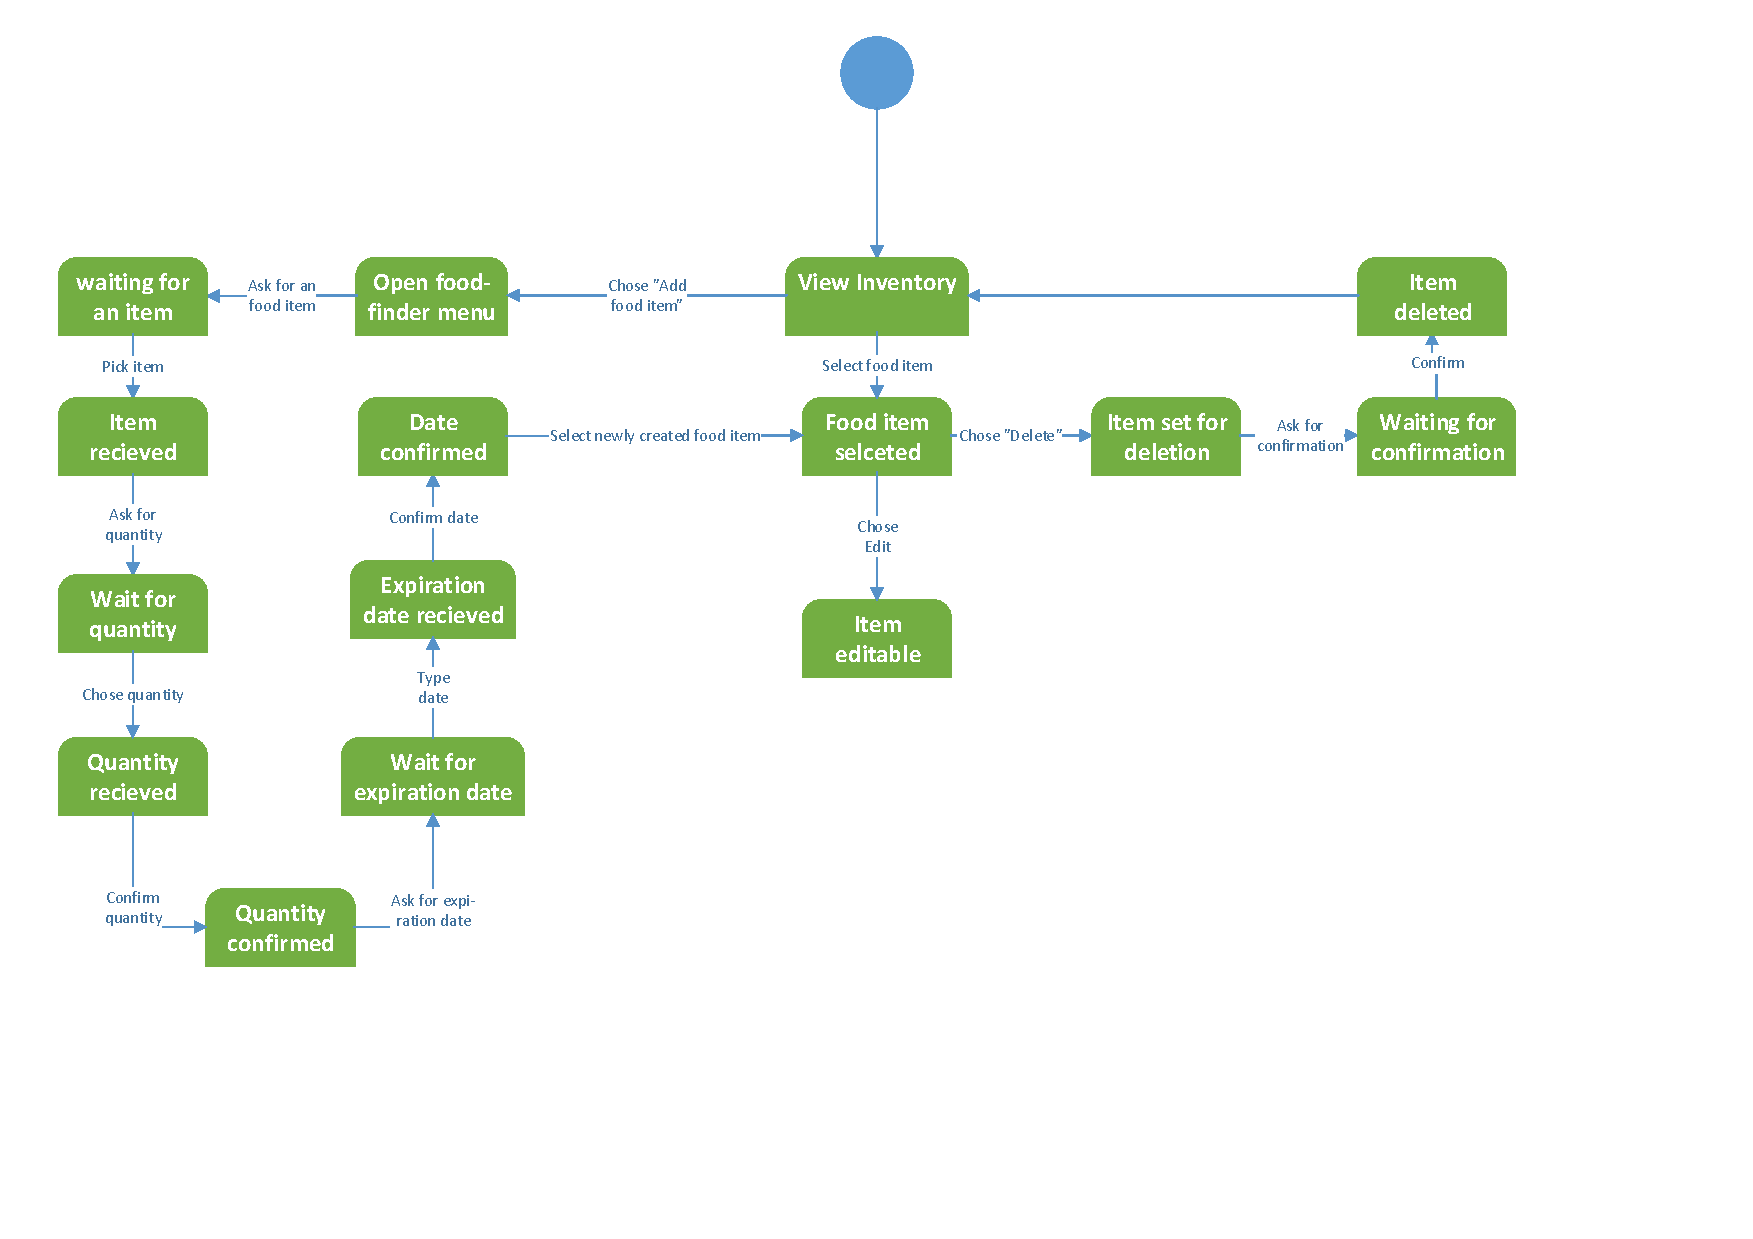
\includegraphics[width=1.0\textwidth, trim= 0 4cm 3cm 0]{ApplicationDomain/spViewInventory.pdf} 
	\caption{The \textit{View Inventory} state diagram}
	\label{Inventory_Figure}
\end{figure}
The user starts on the \textit{View Inventory} state where the inventory is shown. From here the user can choose from three different options: One that adds food to the inventory, another which allows the user to delete existing food items and a last option for editing food items. The edit option has its own diagram (see \cref{spEditInventory}). If the user chooses to add food, they will have to select food from a list. After a food item have been chosen, the system will ask for the user to select a quantity in order to know how much of the food item the user have acquired. For example, the user can buy five bananas or two hundred grams of flour. The user will afterwards have to enter when the food expires. When this is done the food will be added to the inventory. This leaves the user at the food item they have added, as if it was selected on the inventory screen. This is the same result as if the user chose to select a food item from the beginning. From here the user will be able to edit or delete a food item. \label{InvDesc}

When the user chooses to delete a selected item, the system will ask for a confirmation before it is deleted. If the user confirms, the system will delete the food item and go back to the view inventory state.


\Cref{spEditInventory}, is the last diagram which also covers the inventory. In this part of the system the user operates as an administrator.

\begin{figure}[H]
	\centering
	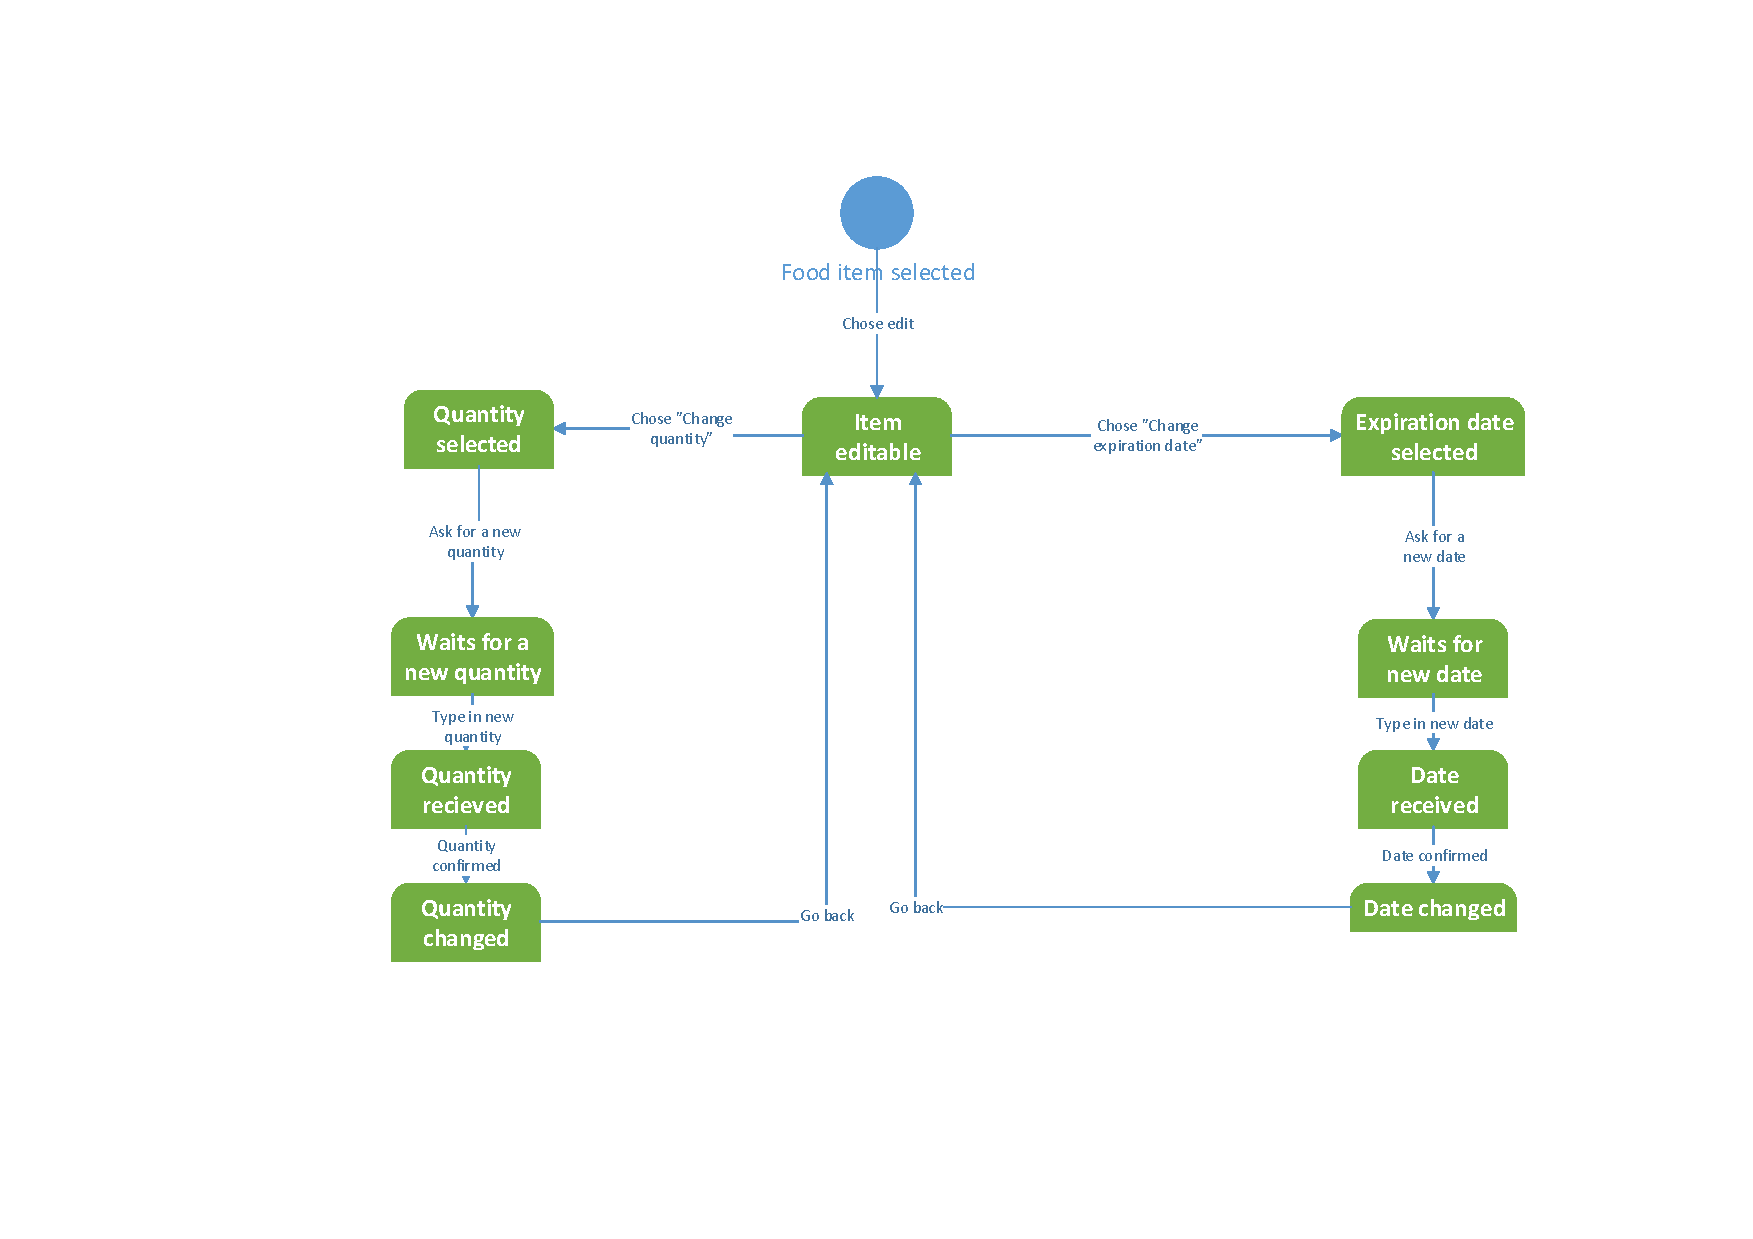
\includegraphics[width=1.0\textwidth, trim= 0 5cm 0 4cm]{ApplicationDomain/spEditInventory.pdf} 
	\caption{The \textit{Edit Inventory} state diagram.}
	\label{spEditInventory}
\end{figure}
The possible options in form of editing, is to change the quantity or expiration date. 
When choosing \textit{Change quantity} it works like the \textit{Change quantity} in the shopping list, which means that choosing an amount that leaves it at zero deletes the item, and leaving it below zero is not allowed. When the user tries to change the expiration date, the system prompts for a new date. All dates will be valid, which means that an item which was expired can go \textit{unexpired} as described at the diagram \cref{MealClass}. This also works the other way around as a fresh item can expire if the date changes to the day prior to the day it expires.

\subsection*{Summary}
The actor specification and use cases helped to establish an understanding of how the user base will interact with the system. By defining the use cases, some flaws in the design were discovered which resulted in varies corrections.
%Funktioner - beskrivelse af systemets funktionalitet se kap 7
%	Komplet funktionsliste
%	Specifikation af funktioner
	
	\chapter{Functions}
	\section{Function definitions}
	The diagrams in \ref{Usage} contain different functions these functions have been given a name and listed in the following tables, where they have been assigned a complexity of Simple, Medium or Complex, and they have been assigned one or more of the following types; Read, Update, Calculate or Signaling. The more complex functions are further elaborated under each table.
\begin{table}[H]
	\centering
	\caption{Shopping list}
	\begin{tabular}{|l|l|l|}\hline
		\textbf{Function}&\textbf{Complexity}&\textbf{Type}\\\hline
	  Update shopping list  &  Complex & Update \\\hline
	  View shopping list    &  Simple  & Read   \\\hline
  \end{tabular}
  \begin{flushleft}
    \textbf{Update shopping list:} The update function will be triggered by the signal function from the inventory "Update shopping list" function". When a meal is added or removed from the food plan. The shopping list should represent what ingredients that is needed to prepare the meals in the foodplan.
  \end{flushleft}
	\caption{Food plan:}
  \begin{tabular}{|l|l|l|}\hline
		\textbf{Function}&\textbf{Complexity}&\textbf{Type}\\\hline
	  Add meal              &  Complex & Calculate, update \\\hline
	  Remove meal           &  Simple  & Update            \\\hline
	  View food plan        &  Simple  & Read              \\\hline
  \end{tabular}
  \begin{flushleft}
    \textbf{Add meal:} The add meal function is given the complex status as it involves many actions in order to add the meal onto the schedule. When the user goes trough the steps necessary to schedule a meal, the system will do a lookup in order to create a list of needed ingredients. This list will be compared with what the user has in the inventory, and any ingredients that is not present on the list will then be added to the shopping list. This is were the previously described function comes into play.
  \end{flushleft}
	\caption{Inventory:}
  \begin{tabular}{|l|l|l|}\hline
		\textbf{Function}&\textbf{Complexity}&\textbf{Type}\\\hline
	  View inventory        &  Simple  & Read   \\\hline
	  Update shopping list  &  simple  & Signal \\\hline
	  Add Item              &  Complex & Update \\\hline
	  Edit Item             &  Complex & Update \\\hline
	  Remove Item           &  Simple  & Update \\\hline
  \end{tabular}
  \begin{flushleft}  	  
    \textbf{Add item:} The add item function have been marked as complex. The function is complex as there many steps involved when adding an item, see \Cref{InvDesc} for a description of these steps. By having this function the user is able to add food to their storage manually.
    
    \textbf{Edit item:} The edit item function is complex as well. If the user changes the expiration date on an item,it could potential update the inventory as an item can "unexpire". The same goes for changing the quantity of an food item. If the quantity reaches zero the item will be deleted, and therefore an update in the storage will be needed.
  \end{flushleft}
\end{table}
\input{ApplicationDomain/UserinterFace}
Den tekniske platform?

%\chapter{Pages}
In this section the documentation and functionality of the different pages will be described, as they are implemented in the program.

\section{Settings} \label{ss:settings}
The settings page allows the user to specify different options for the program. The options are categorized as User Specifics, Stock Management, Rated Ingredients, Unwanted Ingredients and Diets.

Under the \textbf{User Specifics} category, you can change the how many persons that lives in the household, which is used as the default value for how many persons a meal should be scheduled for. You can also select how many days you want to shop ahead for, which means how many days in the future the shopping list takes into account. Finally you can select the default page, which the program shows when started.

The \textbf{Stock Management} category allows the user to add ingredients that they always want to have a specific quantity of. By typing the ingredient into a textbox with auto-completion as described in \cref{sec:AutoComplete} the user can select the ingredient. In the stock list the added stock ingredients are shown and the quantity can be changed by using numeric up-down control. The ingredient can be removed by selecting them and clicking the remove button symbolized with a minus (-) sign.

\textbf{Rated Ingredients} works the same way as \textbf{Stock Management} when adding an ingredient, but instead of setting a quantity, the user can give the ingredient a rating from 1-100 in order to prioritize the search, as described in \cref{ssc:graylist}. The user can also remove the ingredients from the rated ingredients list.

\textbf{Unwanted Ingredients} is similar to \textbf{Rated Ingredients} but the ingredients you add will instead be "blacklisted", as described in \cref{ssc:blacklist}, and thus completely remove recipes with these ingredients from the search.

\textbf{Diets} allows the user to choose a diet, which will make the search prioritize recipes that does not contain specific ingredients, so the user can keep a specific diet. The diets are pre set and can not be changed by the user.

\section{Inventory} \label{ss:inventory}
The inventory page displays a list of the ingredients that the user have in the household. Initially the users sees all the ingredients from the inventory grouped by name, displaying the total quantity of each ingredient and how many individual ingredients there are. By expanding an ingredient with an expander control, the user can see the individual ingredients and change the quantity and expiration date.

In the top the users can add ingredients using the auto-complete control described in \cref{sec:AutoComplete}, which finds available ingredients from the database. The list is initially sorted by name, but can also be sorted by quantity or expiration date.

\section{Shopping List}
The shopping list page shows a list of ingredients that needs to be bought for the recipes in the meal plan within the shop-ahead period mentioned in \cref{ss:settings}. It displays ingredients and the quantity that is missing from the inventory, according to the meal plan and stock management settings. Each ingredient has a check-box so the user can add the selected ingredients directly to the inventory after shopping.

\section{Meal Plan}
The meal plan shows a week of scheduled meals, and allows the user to navigate to the previous and next week. The weekdays are listed as rows, with seven individual lists of meals belonging to the specific days. By clicking the meals the  user can navigate to the Recipe Page to see information about the recipe and/or update meal information.

\section{Search}
The Search page lists recipes sorted by multiple factors, first the Search is sorted by percentage of how many of the ingredients in the recipe the user has in the inventory, then the application sorts the list by the number of ingredients the user has partially in their inventory. Then the application sorts the search results by the rating of the ingredients in the recipe, then by how many times the ingredients in the recipe has been used in the past. Lastly the search results are sorted by the name of the recipe.
In the top it is possible to search for recipes by searching for the recipe name, or ingredients sorted by comma.

\section{Recipe Page}
The recipe page shows information about a recipe or meal. By clicking a recipe in the search, you navigate to the recipe page which displays the title, image and description of the recipe as well as a list of ingredients. In the top you can add the recipe to the meal plan, and if it is already added you can update the date, or remove the recipe from the meal plan.
By clicking a meal on the meal plan the user is also taken to this page.


\chapter{Problem Statement}
It is a problem that so much food is going to waste. This is a consequence of bad planning when people are shopping for their upcoming week, and because the consumers want fresh groceries. Miscalculations are bound to happen if the one doing the shopping is part of a bigger group, such as a family. Shopping is also time consuming if people want their groceries at a low price. It can be hard to balance the price and time if the cheap stores are far away, or if the consumer is unaware of recent discounts. It becomes extra time consuming if the shoppers have special food diets or preferences. Users who live alone also find that they have a big foodwaste, and have a higher cost per meal than users who live and eat together with others. The problemst that was found can be summed up to the list:

\begin{itemize}
    \item Too much food is being wasted.
    \item Micalculations happen when more people live and eat together.
    \item Shopping is time consuming.
    \item Diets is hard to take into consideration.
    \item Consumers living alone have the biggest foodwaste per person.
    \item Consumers living alone have a higher cost per meal, that people living with others.
\end{itemize}

\textbf{How is it possible to create a software solution that caters to the needs of those who wants to save resources, but still maintain a low foodwaste level, and still want to be able to fulfill their food lifestyle choices.}

%How can a software solution make it possible to plan ahead and also take into consideration any relevant kind of special requirements that the user has.